\hypersetup{pdfborder=0 0 0}
%\vspace{10\baselineskip}


%\selectlanguage{french}


\section{Résume en français}



%-------------------------------------------------------------------------------------
%\color{blue}\section{3D LES in the Strait of Gibraltar} \color{black}
\section{Introduction}

The Atlantic - Mediterranean exchange occurring in the Strait of Gibraltar has been \color{blue} explored \color{black} summarily in a previous section (2D \color{blue} Utilise des labels dès maintenant pour les sections et les sous-sections cela t'évitera de perdre du temps à tout vérifier et tout reprendre à la fin \color{black}). \color{blue} The consequences at basin scale broadly \color{black} consists in Mediterranean waters leaving the Strait at depth (as what has been dubbed the 'Mediterranean outflow') whereas \color{blue}Atlantic\color{black} waters enter the Mediterranean basin in the surface layer.

Those Atlantic waters entering through Gibraltar strait are the principal contribution to the Mediterranean inflowing water budget: the average transport of Atlantic waters at \color{blue}Gibraltar \color{black} is of the order of 1 Sv whereas tshe net exchange itself is of the order of 0.1 Sv. \color{blue} This positive entry offsets the otherwise net evaporation occurring on the integrated surface \color{blue}over \color{black} the Mediterranean basin \citep{bryden_1994}.
Since the Mediterranean basin is otherwise a closed basin, Mediterranean waters leaving the strait of Gibraltar are the result of the transformations \color{blue} of the Atlantic water mass \color{black} into intermediate and deep water masses\color{blue}\sout{ of the Atl waters that circulated in the Mediterranean} \color{black}.
More details are provided in this section on the characteristics of the strait, \color{blue} on the exchange and variability and on the fine-scale processes that take place during this exchange \color{black}.



\subsection{Circulation in neighbouring areas (Gulf of Cadix and Alboran Sea)}

 \color{blue}\sout{(de Pascual-Collar ; NAjanro 2012 ; Sanchez Garrido 2013 ;Lorente 2019 ; garcia lafuente 2017)} 
 \color{black}

\textit{Atlantic side \color{blue}of the strait of Gibraltar \color{black}}

The surface waters that end up entering the strait are \color{blue} North Atlantic Central Water (NACW) \color{black} and South-Atlantic Waters (SAW) \color{black} \citep{millot_2014,naranjo_2015}. They are carried by the Portugal and Azores Currents into  \color{blue}Gibraltar strait \color{black} as part of the eastern branch of the north-Atlantic subtropical gyre \citep{barton_2001}.

Below this surface circulation \color{blue} in the Northern Atlantic\color{black}, can \color{blue}be found \color{black} the Mediterranean outflow, \color{blue} i.e. \color{black}the Mediterranean water mass that was transported out of the strait by the Mediterranean outflow. \color{blue}This outflow first enters \color{black} the Gulf of Cadix,  \color{blue}turning \color{black} north due to geostrophy and flowing along \sout{the bathymetry of} the continental slope \citep{price_1993,gasser_2017}. 

\color{blue} West of the Gulf of Cadiz, it \color{black} stabilizes to its neutral buoyancy level at \color{blue} 1000-m deep \color{black} as the "Mediterranean water mass"\citep{price_1993}. Meddies, salty lenses of water with negative  \color{blue}(?) \color{black} vorticity \sout{able to} \color{blue}can  \color{black} persist for years \sout{that are} \color{blue} and can be found \color{black} far in the open ocean. \color{blue}They \color{black} are generated along the canyons and caps encountered by the Mediterranean outflow in the region of the Gulf of Cadiz \citep{bashmachnikov_2015}. The Mediterranean outflow itself participates in the global circulation \color{blue}in the \color{blue}northern Atlantic \color{black} overturning circulation \color{blue}(?) \color{black} \sout{by salinification of the overall}. \color{blue} It increases the salinity of the whole Northern Atlantic basin as the Mediterranean water mass spreads in the open ocean, as meddies decay but also as this outflow join the basin scale circulation at higher latitudes. \color{black} \citep{price_1993,jia_2007}.\\


\color{blue}\textit{Mediterranean side of the strait of Gibraltar} \color{black}


Surface waters leaving the strait at the east enter the Alboran Sea as the Atlantic Jet (AJ). The circulation of the Alboran sea \color{blue}can vary in time\color{blue}. The most common state is organized around two anticyclonic gyres: \color{blue}the Western Alboran Gyre (WAG) and the Eastern Alboran Gyre (EAG)\color{black}. \color{blue}However, it is \color{black} not uncommon that only one of \color{blue}these two gyres \color{blue} is present \citep{millot_2005}. The WAG is coupled to the Atlantic jet \color{blue}and \color{black} usually constitutes its northern branch, \color{blue}whereas the \color{black} variability of the AJ is mainly due to meteorological and tidal forcing which can destabilize this system \citep{sanchez-garrido_2013,lorente_2019}.

At depth, several \color{blue}components of \color{black} the Mediterranean water masses enter the strait. In the Alboran Sea, \color{blue}they are \color{black}identified as LIW (for Leventine Intermediate Water) and WMDW (for West Mediterranean Deep Water). \color{blue} Additional water masses from the western Mediterranean basin \color{blue} like TDW (for Thryenian Deep Water) \color{blue}have \color{black} being detected \color{blue}(Millot ?)\color{black}. \sout{There is a south/north repartition of those watermasses} A zonal organization of these water masses has been observed: TDW, LIW and other intermediate waters are \color{black} more abundant in the northern part of Alboran sea, whereas WMDW  \color{blue}is mostly present \color{black} in southern part \citep{millot_2014}. As the depth decreases from the Alboran sea to the strait, it is more difficult for deeper WMDW to \color{blue}pass through the \color{black} strait, and the flow can be regulated by mechanisms such as the strength of the WAG or the overall production of WMDW linked to winter convection (Najanro 2012).\\


\color{blue}\textit{Transformation of the water masses.} \color{black}

\color{blue}Both the inflowing (in reference to the Mediterranean basin) Atlantic waters or the outflowing (ditto) Mediterranean waters incorporate \color{black} signatures of respectively the Mediterranean (Macias 2006) and Atlantic waters (Millot, 2006, GarciaLafuente, 2011). This is due to the mixing driven by small-scale processes of variable strength \color{blue}occuring in the strait of Gibraltar. \color{black} 


%%%%%%%%%%%%%%%%%%%%%%%%%%%%%%%%%%%%%%%%%%%%%%%%%%%%%%%%%%%%%%%%%%%%%%%%%%%%
\color{blue}\subsection{Morphology, barotropic tides and atmospheric forcing.} \color{black}
%%%%%%%%%%%%%%%%%%%%%%%%%%%%%%%%%%%%%%%%%%%%%%%%%%%%%%%%%%%%%%%%%%%%%%%%%%%%%


The Strait is \color{blue} tilted at approximately \color{black} 15$^\text{o}$ in the east direction. Away from \color{blue}the continental shelf \color{black}, Camarinal Sill (CS) the shallowest point with \color{blue}an average depth of about 300 m. In the region of CS, the strait is also narrower but deeper on the Mediterranean side. \color{black} On the Atlantic side now, it is shallower, with two troughs on each side of a submarine mount called Majuan Bank. The northern trough is shallower than the southern one, which includes another sill, called Espartel Sill (ES). Those two troughs are the main pathways the \color{blue}Mediterranean outflow takes \color{black} to \color{blue} reach \color{black} the gulf of Cadix. Most of the flow takes the southern deeper path \color{blue}(only 18 \% of the water mass flows north (Soto-Navarro 2014)\color{black}.

The barotropic (M2) semi-diurnal tide \color{blue} flows \color{black} from the North Atlantic \color{blue}basin and constitutes \color{black} the foremost varying signal for the currents in the strait, propagating from south to north with an amplitude decreasing from west to east\citep{candela_1990}. During the flood (ebb) tide, barotropic currents are oriented westward (eastward). The currents associated with the barotropic tide \color{blue} have the \color{black} same amplitude as the mean circulation\color{blue}. They \color{black} can reverse the flow of Mediterranean and/or Atlantic waters in certain sections(Sanchez Roman 2012), and they have a pronounced neap-spring tide cycle.

The wind is funneled through the strait and is either \color{blue}blowing westward or eastward and it is \color{black} principally zonal (?) with a speed \color{blue}reaching \color{black} $25\ m/s$ (Candela 1989). Wind stress affects only the first tens of meters of the circulation in the strait (Candela 1989), which can be sufficient to affect the Atlantic jet, by \color{blue}inducing either an acceleration (and a change of direction when leaving the Strait) or a deceleration (sometimes even stopping the jet) \color{black}(Lorente, 2019). Otherwise, the integrated effect of atmospheric pressure over the Mediterranean basin \color{blue} can \color{black} influence the net flow through the strait (Garcia Lafuente 2002).



%%%%%%%%%%%%%%%%%%%%%%%%%%%%%%%%
\subsection{Baroclinic exchange and small-scale processes}


The circulation of eastward Atlantic waters at the surface and of westward Mediterranean waters at depth sets up a baroclinic exchange in the strait of Gibraltar. Due to the amplitude of the barotropic \color{blue}(tidal) currents, this exchange is \color{black} intermittent with regard to the M2 tide. \color{blue}The circulation can thus be splitted into a Reynolds-averaged sheared component and a depth-averaged, eddy-flux-like anomaly. The latter has an important impact on the exchange flow (Naranjo, 2014, etc..), and can even have a larger amplitude than the former at CS (Vargas, 2006). \color{black}
\sout{One can thus see the exchange as a Reynolds(?) decomposition of an average with tidal contribution as eddy-fluxes that impacts secondary characteristics of the exchange (Naranjo 2014, etc..), and which have a more important amplitude at CS (Vargas2006).}  

\color{blue}The amplitude of the exchange varies \sout{with other} over timescales larger than the semi-diurnal tide. The lower frequencies (whether seasonal or inter-annual) are usually linked to atmospheric forcing over the Mediterranean (SanchezRoman2012?). \color{black} The tidal eddy-fluxes have their own variability associated to the spring-tide cycle and to the monthly tides, with for example a greater depth and stronger shear during neap tides, but more intense mixing during spring tide (Naranjo 2014, Vargas 2006).

\sout{Behind those characteristics varying at the tidal time-scale} \color{blue}Various small-scale processes can additionally be identified in the Strait of Gibraltar. \color{black}

Firstly, due to the limited horizontal and vertical extent of the strait, \color{blue} the time-averaged exchange flow and the depth-averaged barotropic tidal currents are channeled in the strait. \color{black} A consequence is that the flow in the strait can become supercritical in regard to internal gravity wave propagation \color{blue} meaning that the velocity of the currents are larger than the velocity of the internal gravity waves. \color{black} East (west) of CS, the flow in the Atlantic (resp. Mediterranean) layer becomes supercritical.
\sout{, although the detail of how regular/their disposition and geometrical extent depends on the framework one uses. (exemples: Farmi et Armer 1988,Sannino 2007,Sanchez Roman 2012,Vargas 2006...) In particular, hydraulic control occurs at Camarinal Sill episodically.}
\color{blue} Hydraulic control of the exchange flow only occurs episodically at CS. More generally, the location and the variability of the occurrence of supercritical flows can yet vary depending on the type of diagnostics used to characterize such events (see for instance Farmi et Armer 1988, Sannino 2007,Sanchez Roman 2012,Vargas 2006...). \color{black}

\color{blue}In the region of CS, the \color{blue} development of two hydraulic jumps reflects the geometry of the sill and can be observed on satellite imagery (brandt1996). The hydraulic jump remains approximately 4 hours in the region of Camarinal during outflows (Vlasenko 2009). \color{blue} During this particular period, an intense mixing of Mediterranean and Atlantic waters occurs (Wesson andGregg; Lafuente...2011,MAcias2006(?)). \color{blue} Strong billows are indeed induced by \color{blue} Kelvin-Helmoltz instabilities in the lee of the hydraulic jump. These bellows are then advected westward by the Mediterranean flow (Wesson andGregg). In addition, Bruno (2013) shows that the establishment of the hydraulic jump matches with the presence of chlorophyll-rich waters in the center of the strait. \color{black}

\color{blue}When the tidal flow reverses toward the Mediterranean basin, the depressed anomaly of the interface between Mediterranean and Atlantic waters propagates as a Large Amplitude Internal Wave (LAIW). It takes the form of a solitary bore before transforming into an Internal Solitary Wave (ISW) (Farmer and Armi 1988). An ISW is a particular type of internal wave satisfying a balance between non-linear advection of momentum and non-hydrostatic dispersion. The consequences of such solitary waves \color{black} have been observed both at the surface and at depth (Ziegenbein (1970), Watson and Robinson 1990,Farmer and Armi 1988,SanchezGarrido 2008,etc.). They transport chlorophyll (Bruno2013) and \color{blue} they are expected to induce \color{black} remote mixing in the lboran sea.

ISWs are generated during each tidal cycle except when westward current are not strong enough  \color{blue}for the hydraulic control to set up. This is for instance the case during neap tide (Watson and Robinson 1990, Garcia Lafuente 2000). When generated, ISWs are refracted as they leaves the strait when the interact with the bathymetry. \sout{either as a curve or asymmetrically with an angle in the north} (?) \color{black} (Watson and Robinson 1990).

\color{blue}The hydraulic control, the hydraulic jump and the generation mechanism of large internal tides can be simulated numerically by hydrostatic models but a non-hydrostatic model is required to simulate the propagation of ISWs or the large turbulent eddies and primary instabilities induced by the baroclinic exchange flow (Brandt 1996; (Vlasenko 2009)). \color{black}



%%%%%%%%%%%%%%%%%%%%%%%%%%%%%%%%%%%%%%%%%%%%%%
\subsection{Discussion}

The small-scale processes are consequently responsible for the mixing of Atlantic and Mediterranean waters in Gibraltar strait, and the characteristics of the water masses involved in the baroclinic exchange at Gibraltar are not conserved (garcia lafuente 2017). \color{blue} \sout{: difficult to link characteristics at ES (INGRES, long term mooring to monitor outflow) to processes in the Mediterranean).} It remains yet difficult to clearly isolate the retroaction of such small-scale processes on the circulation and more generally on the large-scale processes observed in the Mediterranean basin  (INGRES?). \color{black}
The enhanced mixing in the strait must in any event be \color{black}parameterized in coarsely-resolved global or even in regional models and the modification of water-mass characteristics \color{black} has an impact on the circulation in both the Mediterranean and the northern Atlantic basins. 


Based on the preliminary numerical study presented by Hilt2020 \color{blue}(chapter XX of the present manuscript), the 3D s-coordinate, non-hydrostatic, free-surface model CROCO is implemented in the region of Gibraltar with a horizontal resolution of a few tenths of meters. We should show that such a high resolution grid is sufficient to resolve at least the largest scales of the mixing processes in the strait, i.e. the largest turbulent eddies or primary instabilities. A specific focus is on the \color{black} different tidal forcing configurations during a neap-spring tidal cycle \color{blue} and on the way the flow characteristics and the intensity of mixing processes are affected by this variability. \color{black}


The numerical simulation framework \color{blue} based on three simulation periods is presented in section \ref{section3Dnum} and the various diagnosis that have been implemented in the numerical experiments are then described (blah) (?) in section \ref{PartDiag3D}. Section \ref{section3DRes} presents results pertaining to the hydrological state of the flow depending on the strength of barotropic tidal currents, the propagation of ISWs, the areas of generation of primary instabilities and a comparison of several turbulence closure schemes.\color{black}






\section{Numerical Configuration}
\label{section3Dnum}
\subsection{Numerical framework}

\color{blue}Numerical configurations are based on \color{black} CROCO-NBQ building on Hilt (2020), see chapter XXX. \color{black} Table \ref{tab_NH-HR} summarizes \color{blue} the main numerical parameters and choices that have been made. A non-linear equation of state and no-slip condition at the bottom have also been implementted. \color{blue} A simple Smagorinsky-like turbulent closure scheme (Smago in Table XXX) has been used except obviously in configurations dedicated to the evaluation of different closure schemes (section ?). The characteristic Smagorinsky coefficient is chosen equal to 0.05 (reference?).\sout{For paragraph ... three simulations use Smago with coefs} In section (XXX), several Smagorinsky coefficients are further tested  ($10{-3}$,$10{-2}$,$10^{-1}$) and the consequences on the dynamics are carefully evaluated together with that of the used of a GLS k-$\epsilon$ turbulent closure scheme. \color{black}

\color{blue}A crucial aspect of such high-resolution numerical configurations of Gibraltar strait is the realism and the quality of bathymetry data. Indeed the topography of the strait has significant (not to say major) consequences on the local and regional dynamics. A 100-m-resolved MNT SHOM bathymetry has been used and adapted to model requirements (figure \ref{FigBathy3D}. (bathy seuillée?) \color{black}

Initialization and open-boundary conditions (which include tidal forcing) are based on a simulation of the operational Med and Black Sea by ENEA using MitGCM (ENEA, Rome)\footnote{http://www.enea.it/it/seguici/pubblicazioni/pdf-volumi/cresco-report-2016.pdf}. This ENEA configuration can be viewed as a parent simulation. \color{black} It has an horizontal resolution in the strait of $\approx$ 700 m with vertical z-levels (repartition? Ref). \sout{, that are interpolated on grid of horizontal resolution 45 m with 40 evenly spaced vertical $\sigma$-levels.} \color{black} As noted in table ..., this is sufficient to be more resolved in the vertical direction than in the horizontal for the whole simulation domain. \color{blue}(???) \color{black} At Camarinal Sill, vertical resolution varies from $\approx$7.5m at the top to $\approx$12.5m downslope. \color{blue}(???) No wind forcing and no atmospheric fluxes are specified at the surface of the ocean in the studied configurations. This choice is not a consequence of any numerical constraints or malfunctions but is dictated by the will to address the complex dynamics of the region step-by-step, concentrating first on the exchange and tidal flow crossing Gibraltar strait and on the fine scales developing at depth in a realistic context (apart from the atmospheric forcing). Complete, realistic configurations (including the atmospheric forcing) are eventually carried out to prepare Gibraltar campaigns, to deliver forecasts during the campaigns and hindcasts to further explore the processes observed during the 2020 campaign.\color{black}

%This choice is dictated by the complexity of the dynamics in the region and the necessity to clearly understand in a first step...
\color{blue}To somehow reduce the computing cost of the various numerical configurations, the first 6 hours can be seen as a spin-up and are simulated with CROCO's hydrostatic kernal over a 50-m-horizontal-resolution grid. The last field is used as a restart file to initialize the fully non-hydrostatic, NBQ simulation. This 6-h spin-up is made necessary by the large ratio existing between the grid length-scale of the MitGCM ENEA coarse-grid field and the CROCO grid length-scale (a ratio reaching 15 to 30 depending on the studied configurations). Such a downscalling procedure should be implemented through a cascade of simulations. On top of the exploration of the fine-scale dynamics and of its retroaction on the larger-scale circulation in the region of Gibraltar strait, the present study is framed in the numerical development of two-way downscalling of this region in basin-scale circulations models.\color{black}

% Otherwise the balance in MitGCM is to coarse for stability at high resolution.

\begin{table}[!h]
        \centering
        \begin{tabular}{|p{\linewidth/3}|c|c|}
                \hline
                Grid Extension & \multicolumn{2}{c|} {6°4.8'W  5°3.4'W ;}\\
                & \multicolumn{2}{c|} {35°23.8'N  36°27.4'N}\\
                Number of horizontal grid points & \multicolumn{2}{c|} {2049x2621}  \\
                Number of vertical $\sigma$-levels & \multicolumn{2}{c|} {40} \\
                $\Delta x = \Delta y$ & \multicolumn{2}{c|} {45 m}\\
                Depth & Min & Max\\
                & 26 m & 960 m\\
                $\Delta$z & 0.7 m & 24 m\\
                Internal time-step ($\Delta t_s$) & \multicolumn{2}{c|} {1 s}\\
                External time-step ($\Delta t_f$) & \multicolumn{2}{c|} {1/11 s (change 1/14)}\\
                Advection scheme & \multicolumn{2}{c|} {WENO-5} \\
                Viscosity $\nu$ & \multicolumn{2}{c|} {10$^{-6}$ m$^2$/s} \\
                Diffusivity $K_\rho$(aussi Ks et Kt) & \multicolumn{2}{c|} {10$^{-6}$ m$^2$/s}\\
                Pressure/accoustic wave speed$C_s$ & \multicolumn{2}{c|} {400 m/s}\\
                Tidal harmonics (from ENEA) & \multicolumn{2}{c|} { $\text{M}_{\text{2}}$, $\text{S}_{\text{2}}$,$\text{K}_{\text{1}}$, $\text{O}_{\text{1}}$ }\\
                \hline
        \end{tabular}
        \captionof{table}{Simulation parameters}
        \label{tab_NH-HR}
\end{table}


\begin{table}[!h]
        \centering
        \begin{tabular}{|c|c|}
                \hline
                Closure scheme & Simulation name\\
                \hline
                Smago 0.005 & SimIT,SimNT,SimST\\
                Smago 0.001 & SimIT-S001\\
                Smago 0.01 & SimIT-S01\\
                Smago 0.1 & SimIT-S1\\
                GLS K-$\epsilon$ & SimIT-Kep\\
                \hline
        \end{tabular}
        \captionof{table}{Simulation names (ou combiner avec tableau d'avant ???)}
        \label{tab_sim3Dnames}
\end{table}


\subsection{Tidal forcing and simulation period}
The tidal forcing is integrated to the forcing \color{blue} at the boundary  \color{black}. As indicated in table \ref{tab_NH-HR}, it comprises four tidal harmonic \color{blue} components \color{blue} ($\text{M}_{\text{2}}$, $\text{S}_{\text{2}}$, $\text{K}_{\text{1}}$, $\text{O}_{\text{1}}$).
%Due to computational cost constraints,
\color{blue}To limit computational costs\color{black}, simulations are run for 3 days \color{blue}during 3 particular \color{black} periods of September, \sout{of year} 2017 (i.e. close to equinox). \sout{The date of the beginning and end} \color{blue}The start and end dates of each NBQ simulation are prescribed in table \ref{tab_dates_MIV}. \color{blue} They do \color{black} not include the 6-hour-hydrostatic spin-up period. The comparison of the sea-level anomaly near Tarifa \color{blue} located at (5.6° West, 36.01° North) \color{black} in both the parent MitGCM and CROCO simulations and the tidal gauge data (from Puertos del Estado) are shown in figure \ref{fig_maree_tar}. \color{blue} The HR CROCO remains close to parent MitGCM simulation except during the neap tide period. \color{black}

\begin{table}[h]
        %\begin{minipage}{.6\textwidth}
        \centering
        \begin{tabular}{|c|c|c|}
                \hline
                Situation & Simulation name & Dates (UTC)\\
                \hline
                Intermediate Tide & SimIT & 10/09/2017 19h00 - 13/09/17 01h00  \\
                Neap Tide& SimNT & 13/09/2017 16h00 - 15/09/17 17h00 \\
                %\hline
                Spring Tide& SimST & 19/09/2017 22h00 - 21/09/17 23h00  \\
                \hline
        \end{tabular}
        \captionof{table}{Périodes de simulation pour les 3 sitituations VE, MM et ME}
        \label{tab_dates_MIV}
        %\end{minipage}
\end{table}

\begin{figure}[!h]
        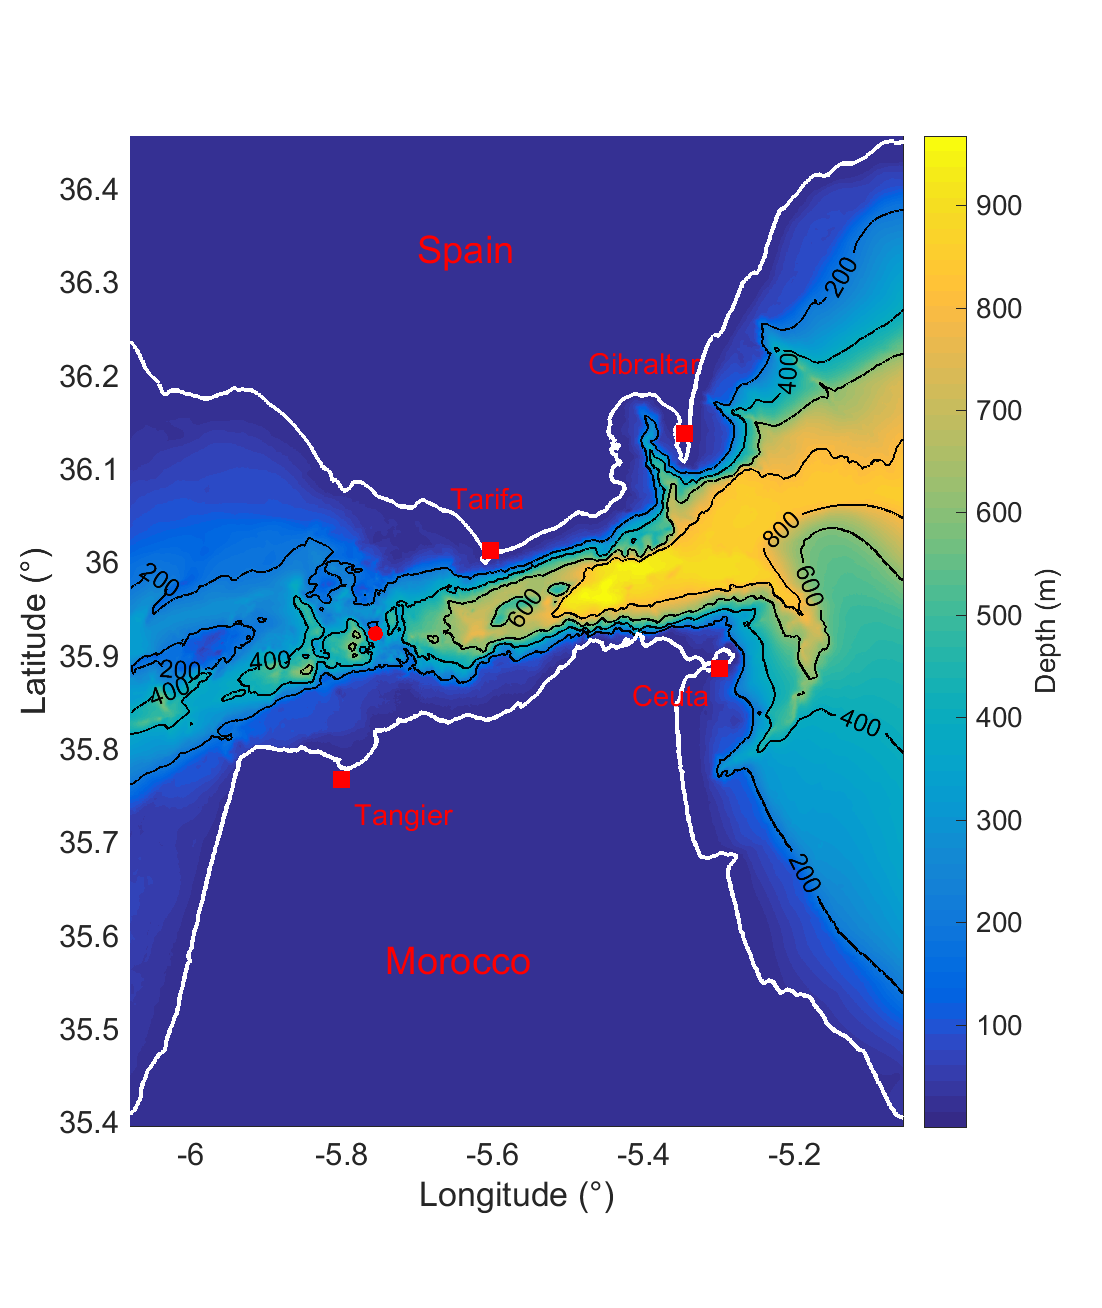
\includegraphics[width=0.5\textwidth]{./GBR3D/FigBathyVHR.png}
        \caption{Area and Bathymetry used for the simulations. The red dot denotes the point at Camarinal Sill where the zonal barotropic current is taken as reference in following figures.  \color{blue}Changer en anglais tangIer \color{black}}
        \label{FigBathy3D}
\end{figure}



\begin{figure}[!h]
        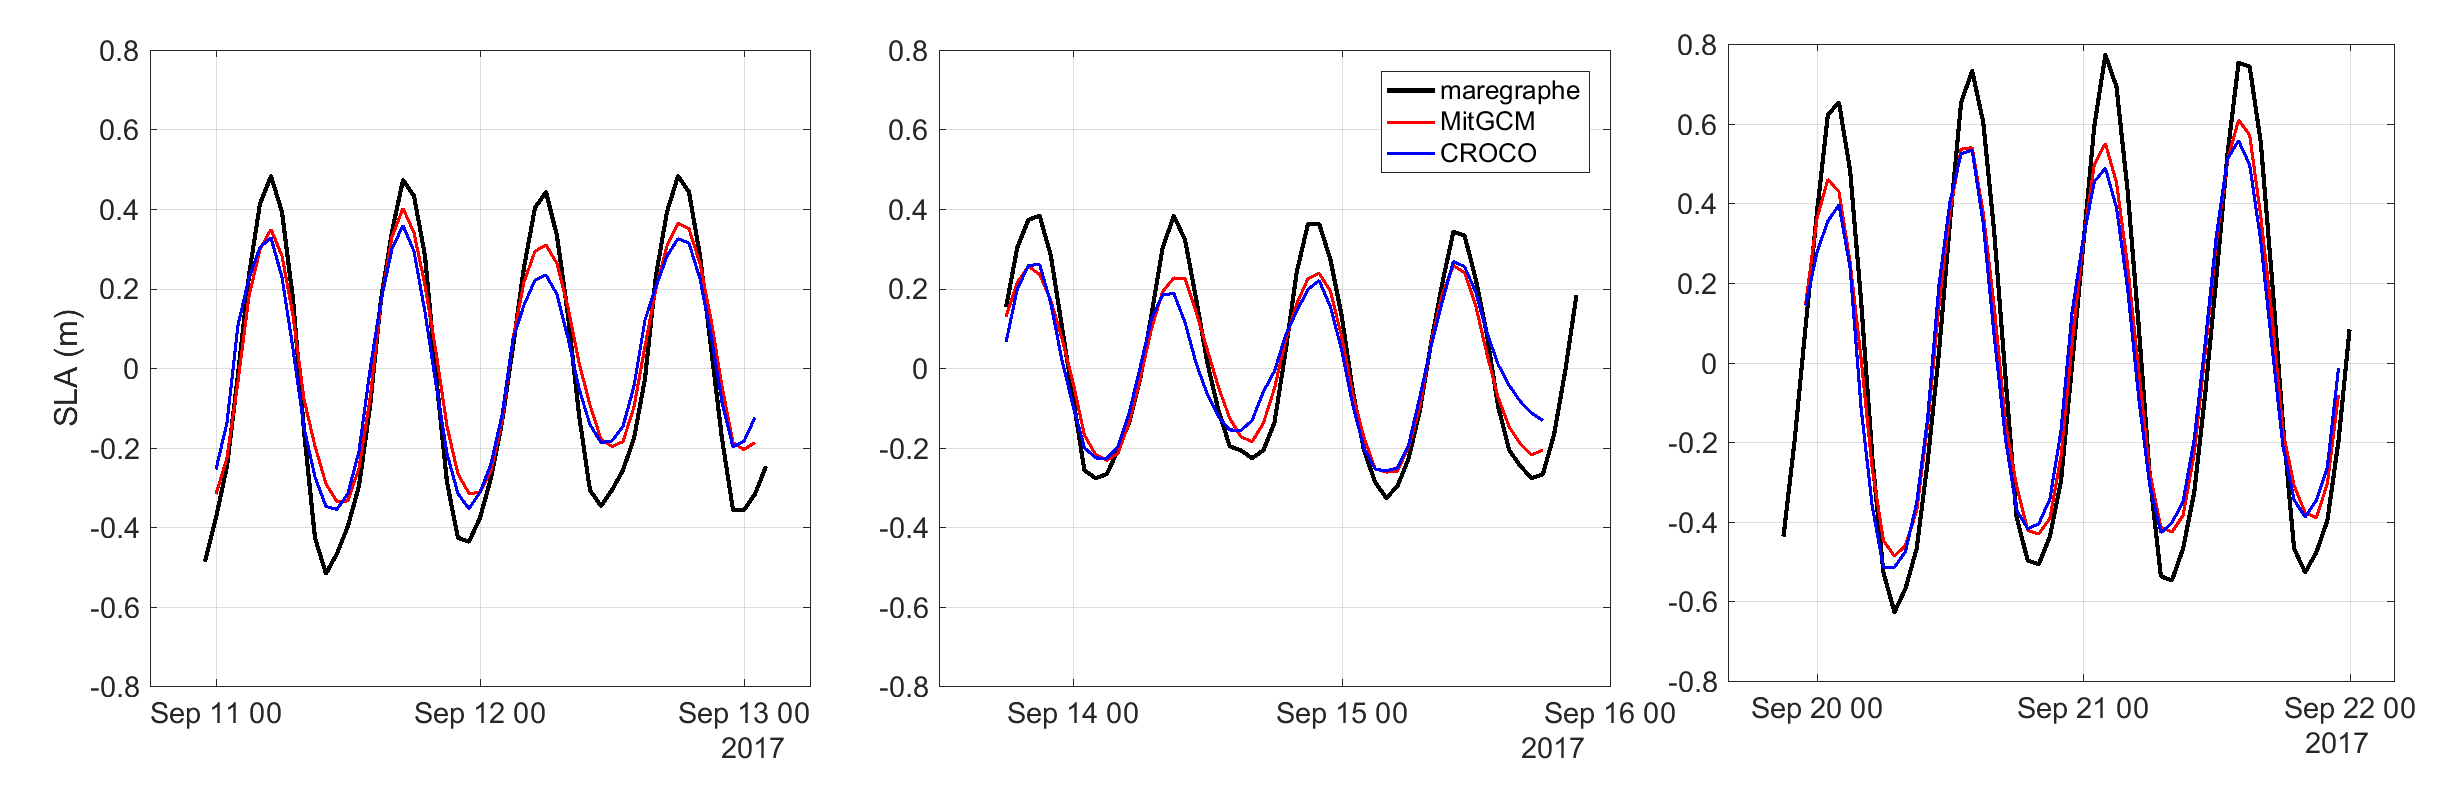
\includegraphics[width=\textwidth]{./GBR3D/SLA_Tarifa_ME2VE2IES.png}
        \caption{Sea level-anomaly at Tarifa from tidal gauge data (black) or at the nearest grid point for parent MitGCM simulation (red) and HR CROCO simulation (blue), for situation ME (a), MM (b) et VE (c)}
        \label{fig_maree_tar}
\end{figure}

\subsubsection{Water masses}
\label{sectionWaterMasses}


\begin{figure}[!h]
        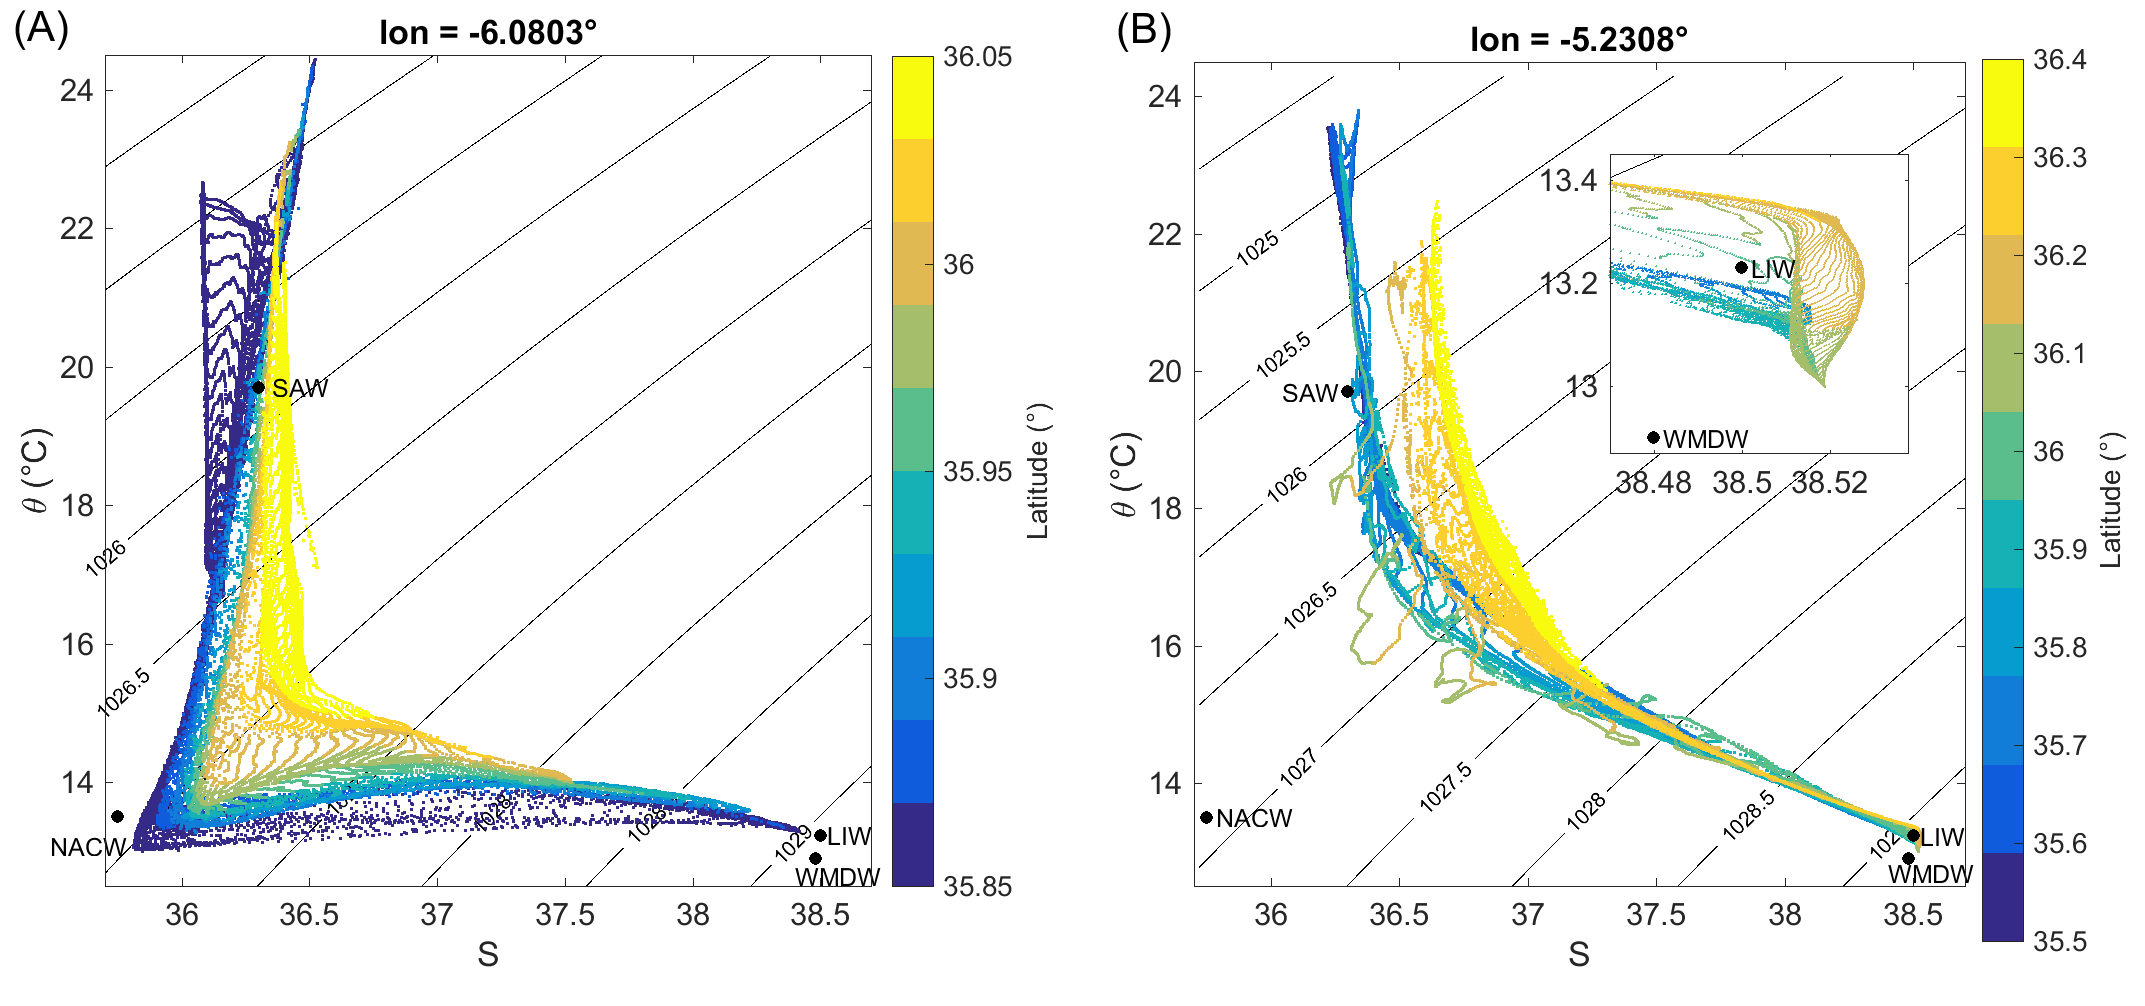
\includegraphics[width=\textwidth]{./GBR3D/WM_ini_IES.png}
        \caption{$\Theta$-S diagrams of grid points at 6.08$^\text{o}$W (a) and 5.23$^\text{o}$W in first timestep of SimIT, color indicates the latitude of each grid point. Cenroid  \color{green} (???) \color{black}definition of certain water masses according to Najanro2014 are also indicated.}
        \label{Fig_Ini_WM3D}
\end{figure}


Figure \ref{Fig_Ini_WM3D} shows the $\theta$-S diagrams for east and west entries of the Strait in  \color{blue}the field of tracers used to intialize the \color{black} simulation SimIT. 
\sout{As expected, for med waters see on the west side two signals for the two pathways of the med outflow, on the east side see distinctly a deep water mass and an intermediate one that could be interpreted as analogous to WMDW and LIW, with the latter being present mostly on the northern part, however in the simulation saltier and warmer waters than expected in bibliography. For atl waters, NACW present on west of domain, less on east.}
\color{blue}At the eastern boundary, the signatures of a deep water mass and of an intermediate water mass that correspond to WMDW and LIW can be identified. The latter is present mostly in the northern part of the domain. The simulated waters are however saltier and warmer than observer water mass (ref XXX).
At the western boundary now, the signature of two Mediterranean water masses corresponding to the two pathways of the Mediterranean outflow. 
As far as Atlantic waters are concerned, NACW are mostly present on the western part of the domain. 
\sout{On east side, see difference surface water north/south of the opening of the Strait, with saltier surface waters in the north. } \color{green} Reformule ou rédige différent, je ne comprends pas ce que tu veux dire...??? \color{black}



\section{Numerical diagnosis}
\label{PartDiag3D}

\subsection{Hydraulic control}
\color{green} 
\textit{Il faut introduire ici les raisons pour lequelles tu as besoin de définir clairement l'interface, ce qui n'est pas évident si tu l'introduit indépendemment de la suite... je te propose donc de regrouper cela dans une section associé au controle hydraulique... .} \color{black}\\

\color{blue}The presence of an hydraulic control is probably the most important diagnostic to be carried out in the region of the strait of Gibraltar. The exchange flow through the strait can shift from a so-called subcritical to critical regime in only a few hours depending on the occurrence (or not) of an hydraulic jump somewhere in the region of the strait. The topography of the region associated to the complex network of pathways for the water masses implies that hydraulic jump can appear and disappear locally. A consequence is that the classification of the whole strait in one "asymptotic" regime or the other is far from simple and probably not necessary.
Diagnostic carried out in the 2D, academic configuration proposed in Section {XXX} consequently need to be refined and, in any case, to be local.\\
To start with, "a" local Froud number needs to be computed and to do so,  the superposition of these Atlantic and Mediterranean water masses (when effective) must be caricatured as a simple two-layer (at most three-layer) representation of the stratification.
In the previous section \ref{sectionWaterMasses}, Atlantic and Mediterranean water masses have been clearly identified based on their temperature and salinity, salinity being probably the most pertinent tracer to differentiate these waters in the region of the strait. 
A two-layer analysis can still be carried in the present, fully-3D , realistic configuration if
\color{black}
\sout{The analysis of simulation result is based on two layer definition of an Atlantic waters layer and Mediterranean waters layer. They are} defined in regard to a reference salinity, with the interface defined as the height of the first water parcel from the top down in the water column for which salinity is above the reference salinity.

The reference salinity is taken as varying along the Strait as a hyperbolic tangent function of longitude centered at the Camarinal Sill to account for the different water mass composition in the eastern and western part of the Strait of Gibraltar. 

\begin{equation}
	S_i(x)=tanh(\frac{x-X_{CS}}{DX})\frac{S_M-S_m}{2}+\frac{S_M+S_m}{2}
\end{equation}
with $X_{CS}=5.75^o$, $dx=0.25^o$, the location and width of the Camarinal Sill in degrees, $S_M=37.39$ and $S_m=37.1$ the max and minimum values taken respectively east and west of the sill.
\color{green}x, DX dans l'équation ? De plus, on réserve normalement ces notations pour les coordonnées cartésiennes \color{black}

%This may not give the perfect interface at any given time...

%\subsection{Froude layer number}

With the atlantic and mediterranean layers defined as above, the Froude layer number for internal gravity waves is computed for \color{blue} a given water column as\color{black}: 

\begin{equation}
F_i=\frac{U_i^2}{g'h_i} , \ \text{with} g'=g \frac{\rho_2-\rho_1}{\rho_0}
\end{equation}
where $\rho_i$ averaged density in layer i,  $U$ is averaged velocity norm over the layer i of height h. If $F_i>1$ say that the flow in layer i is supercritical.


\subsection{Hydraulic Jump detection, acceleration of flow}
\color{blue}The necessity not only to caricature the stratification but also to evaluate a local phase velocity of internal waves based on this stratification renders the evaluation of a local Froud number rather complex and, as a consequence, can somehow blur the characterization of the local regime of the dynamics.  \color{black}
A simple diagnosis for detection of the hydraulic jump at Camarinal Sill in the simulations is \color{black} now proposed based \color{black} on the impact such a structure has on the flow. 
\begin{figure}[!h]
 \centering
 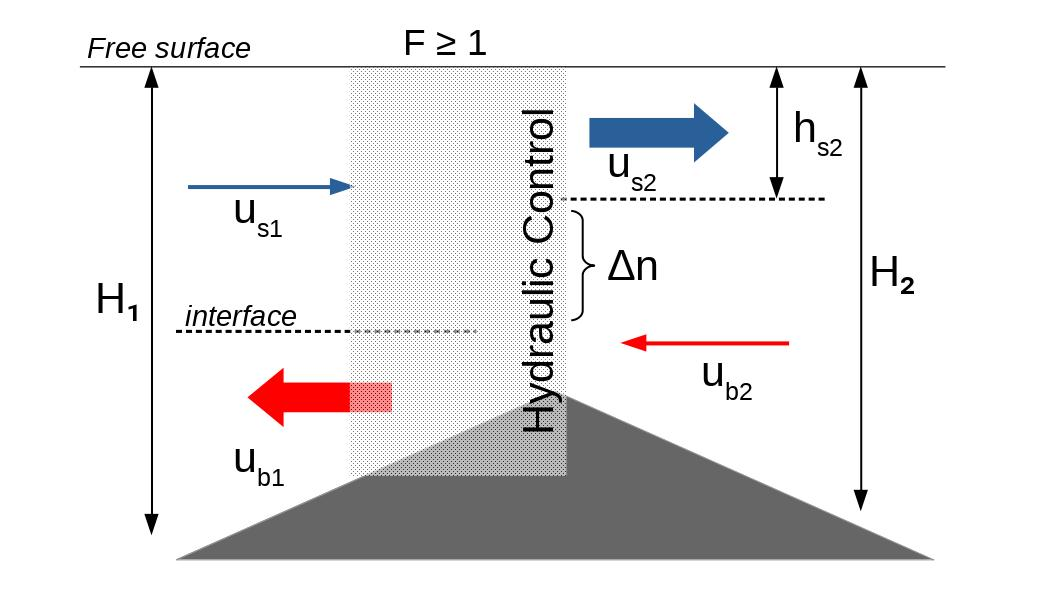
\includegraphics[width=0.5\textwidth]{./GBR3D/schema_diagressaut.jpg}
 \caption {Schematic of flow upstrean and downstream of hydraulic jump at Camarinal Sill in the Strait of Gibraltar.}
  \label{schemaRH}
\end{figure}
As schematized on figure \ref{schemaRH}, an hydraulic jump (also called hydraulic drop) induces a drop of the interface depth. Since the flow in the Strait is canalized by the bathymetry (for the Mediterranean flow) and the coast (for the Atlantic flow), there must be conservation of the flux from \color{blue} a downflow section to an upflow section \color{black} of the hydraulic jump. The variation of the interface depth is indeed associated to an acceleration or a deceleration of the flow (depending on which layer is \color{blue}chosen as a \color{black}reference).
\color{green}Je pense qu'il faut changer les notations et conserver plutôt $h_*$ pour les épaisseurs plutôt que b souvent utilisée pour la flottabilité, n pour une numération entière." \color{black}
The drop in the interface depth is noted $\Delta n=b_2-b_1$, the variation of bottom depth $\Delta H=H_2-H_1$ and the acceleration in the bottom layer $\Delta u_b = u_2-u_1$. In the bottom layer, the conservation of flux is :
\begin{subequations}
\begin{alignat}{2}
  \displaystyle
&u_1 (H_1-b_1)&& = u_2 (H_2-b_2)\\
& &&= u_1 (\Delta H + \Delta n) + u_1 (H_1-b_1) + \Delta u_b (H_2-b_2)
\end{alignat}
\end{subequations}

\begin{equation}
\Delta u_b = -u_1 \frac{\Delta H + \Delta n}{H_2-b_2}
\end{equation}

For the surface flow:
\begin{equation}
\Delta u_s = - u_1\frac{\Delta n}{b_2}
\end{equation}

The velocity in the area of the hydraulic jump must validate the condition of (at least) critical flow, i.e. Froude number $\geq$ 1 at the shallower location. A minimal condition for hydraulic jump is consequently $F=1$, or $U=c$, that is the flow velocity equals the phase speed of internal wave. If, for the latter, \color{blue} an expression for $u_1$ we is given the definition of interfacial velocity: 
\begin{equation}
|u_1|=c=\sqrt{g' \frac{(H_1-\Delta n - b_2)(\Delta n + b_2)}{H_1}}
\end{equation}
 \color{green}Il faut que tu expliques un peu plus ce qui suit... difficilement reproductible par un lecteur qui découvre ce diagnostique. \color{black} 
Several parameters are chosen as threshold, here take values that should be correct for area of camarinal sill, the minimum excursion of the jump $\Delta n = 30m$ and the height of the Atl layer $b_2=50 m$ , and the reduced gravity $g'=0.02 m s^{-2}$.

\subsection{Q parameter and derivated diagnosis}

\color{blue}The studied configurations are all based on grid resolutions of a few tenths of meters, an objective being the explicit simulation of at least the largest turbulent eddies. The region of the Mediterranean outflow is of particular interest since in this region large velocity shears are associated to large vertical density (salinity) stratification.\\
A diagnostic is now proposed to "detect" the primary instabilities and more specifically Kelvin-Helmholtz instabilities developing potentially in this region.
\color{blue} A careful inspection of the relative-vorticity vector can fulfill this purpose and a dedicated scalar diagnostic based on the components of this relative vorticity is retained. It is a generalization of the Okubo-Weiss parameter retained in Hilt (2020) to the present 3D realistic configurations. \color{black}
%A simple vorticity diagnosis is not chosen as it requires choosing the rotation axis, but also because regions of high shear such as between the MEd outflow and Atl waters will have high vorticity values. Instead, analogously to the use of the Okubo-Weiss parameter in Hilt 2020, we chose to compute parameter Q, defined as (ref):
\begin{equation}
Q=-\frac{1}{2} \frac{\partial u_i}{\partial x_j} \frac{\partial u_j}{\partial x_i} = \frac{1}{2} (\Omega_{ij}\Omega_{ij} - S_{ij} S_{ij})
\end{equation}
with $u_i$ the components of velocity vector, and $S_{ij}$ and $\Omega_{ij}$ are respectively the strain-rate tensor and vorticity tensor. When $Q>0$, rotation is predominant over shear part.
 \color{green}Attention à la cohérence des notations ui etc... tout au long du manuscrit. $\Omega$ est en particulier déjà utilisé pour la rotation de la terre, $\omega$ est plus courant pour la vorticité.\color{black}\\

\color{green} Beaucoup trop tôt je pense pour le paragraphe suivant... A ce stade, tu introduis tes diag et éventuellement approches statistiques rendues nécessaires par les configurations auxquelles tu t'attaques. Place-toi si possible dans un cadre un peu plus général. \color{black}
\sout{Due to advection by the Med outflow, a succession of primary instabilities will propagate over teh same grid cells.} The temporal evolution of Q over such grid cell will show oscillations between high positive value (center of a billow/vortex) and low negative values (shear between two consecutive billows). A proxy to detect this area is chosen as high value of standard deviation of parameter Q, as defined in equation \ref{eqstdQ} where the over bar denotes temporal average over 30 minutes, a period over which there will be minimal modification of the general flow in the Strait.

\begin{equation} 
\label{eqstdQ} 
    std ( Q ) (\vec{x},t)=  \sqrt{   \overline{Q (\vec{x},t)^{2}} -  \overline{Q(\vec{x},t)}^{2}  }
\end{equation}

To create 2D maps presented in next section, only the maximal value of standard deviation in the water column is saved...
By implementing this calculation directly in the code, we can asses where instabilities/vortexes propagate without having to make a huge volume of simulation outputs over the whole domain, those economising in storage place and data readability. 

The result of this proxy can be compared to the result of the Singular Value Decomposition (SVD) of the time-varying 3D field. However this calculation is off-line and necessitates a high frequency 3D output to pick up the relevant structures.



\section{\sout{Results} Fine scales in the strait of Gilbraltar}
\label{section3DRes}

\subsection{Flow criticality/Hydraulically controlled layer and hydraulic jump, neap-spring tide variability}


\begin{figure}[!h]
 \centering
 
 \begin{subfigure}{\linewidth}
\centering
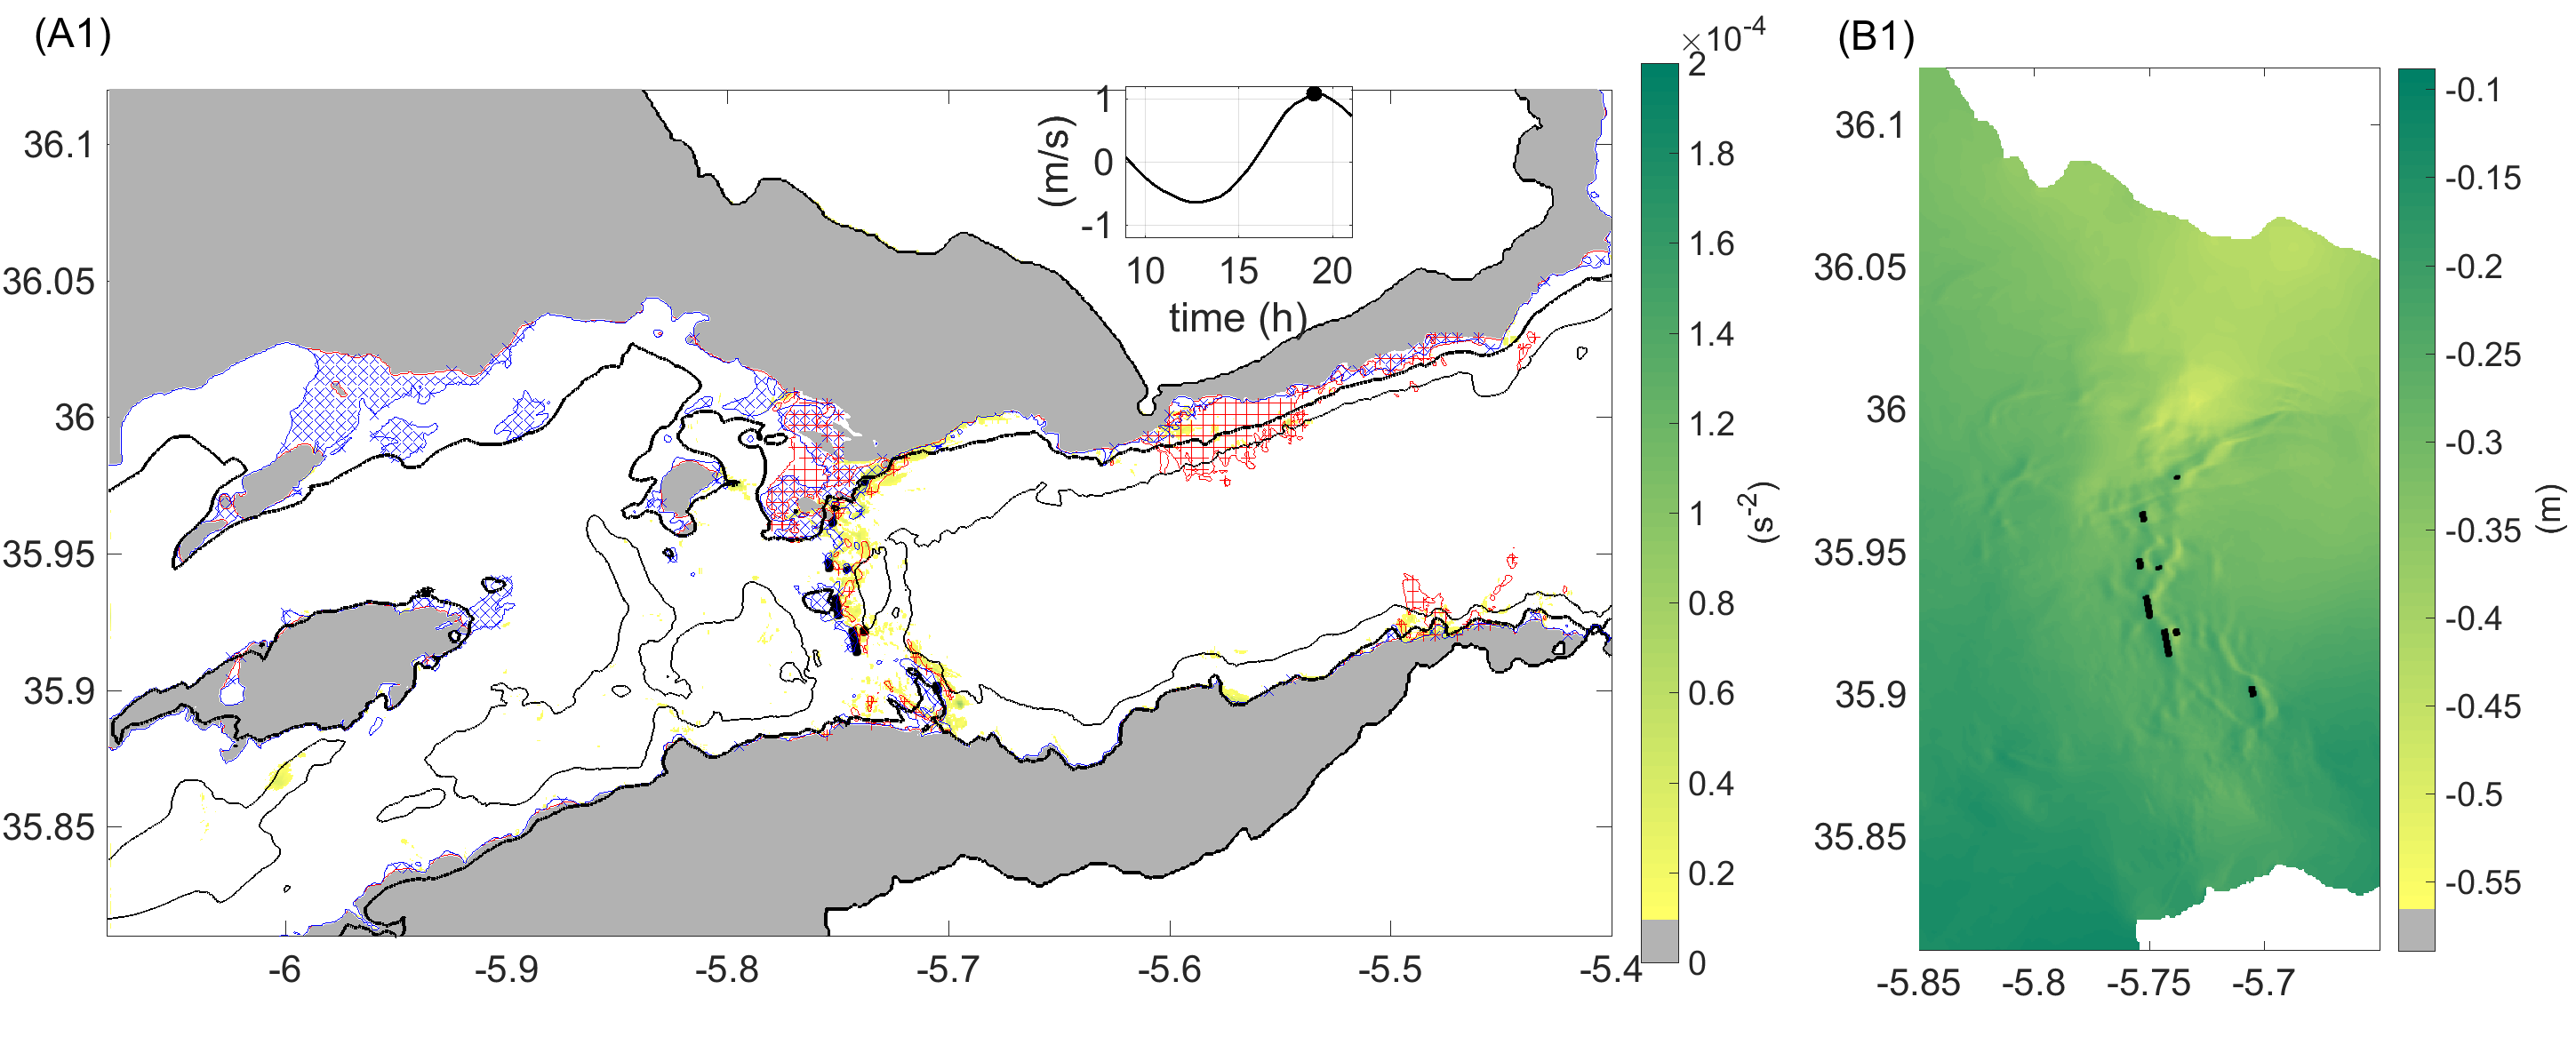
\includegraphics[width=1\linewidth]{./GBR3D/ME2_19h_p.png}
\end{subfigure}
 
 \begin{subfigure}{\linewidth}
\centering
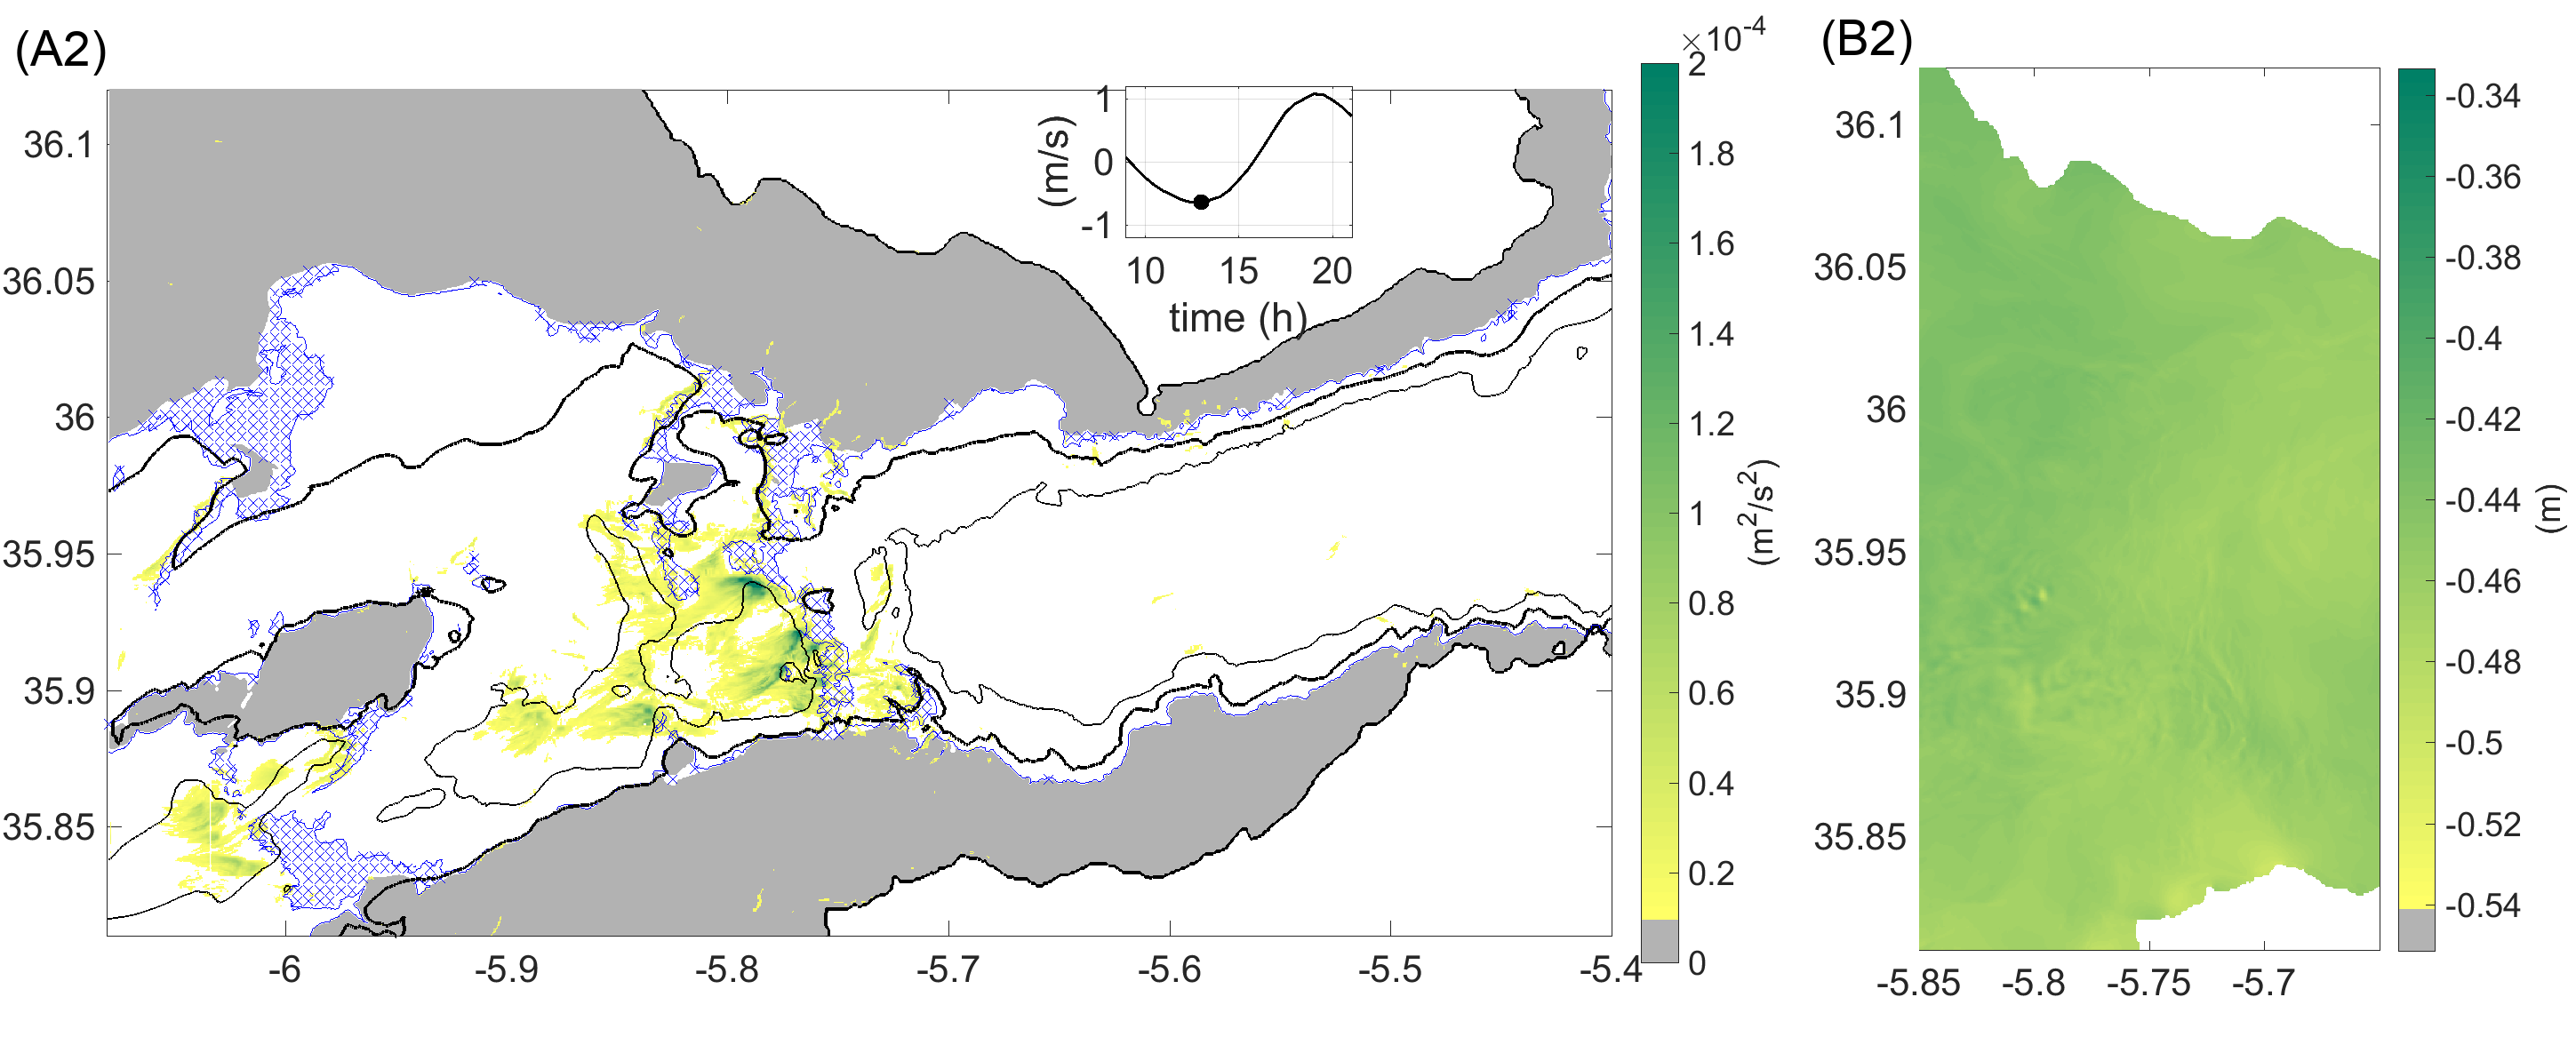
\includegraphics[width=\linewidth]{./GBR3D/ME2_13h_p.png}
\end{subfigure}
\caption {For simulation SimNT, an inflow then an outflow of type \textit{no-jump}. Blue (red) shaded area is supercritical med (atl) layer. Black dots are hyd jump detection. grey area denotes where S bottom$<$Sinterface. colorbar for standard deviation of parameter Q (only values above $10^-5$are represented). Also inicated barotropic znal current at CS (point indicated in figure \ref{FigBathy3D}). Two black isobathes contours are indicated, 200m (bold) and 400m(thin) depth  }
\label{FigHCN}
\end{figure}

Figures \ref{FigHCN} to \ref{FigHCI} present several diagnosis for a series of maximal outflows and inflows \color{blue} presenting \color{black} variable strengths of the tidal forcing among simulations SimNT,SimST and then SimIT \color{blue}Table (XXX) \color{black}. Are represented the diagnosis presented in paragraph \ref{PartDiag3D}: \color{blue}the shaded regions correspond to areas of supercritical flows (\S XXX) in either the Atlantic or Mediterranean layers on top of which are indicated the locations of hydraulic jumps (\S XXX) together with the areas of large standard deviations of parameter Q (\S XXX) (potentially associated to propagating primary turbulent eddies). \color{black} The grey area indicates where the salinity in the bottom level is below the interfacial salinity as defined in \S XXX, and thus \color{blue} where Atlantic waters exclusively are present in the water column. \color{black}

Figure \ref{FigHCN} presents a \color{blue} 'neap-tide' situation \color{black} of weak barotropic currents ($<1\ m/s$ at a shallow point of Camarinal Sill) in \color{blue} both outflow and inflow conditions\color{black}. Figure \ref{FigHCS} \color{blue} corresponds to \color{black} strong barotropic currents ($\geq 1.5\ m/s$) in inflow and outflow conditions during a "spring-tide" period. Finally, figure \ref{FigHCI} corresponds to a period of outflow with intermediate-strength ($\approx 1\ m/s$) of the barotropic currents. \color{black}

\begin{figure}[!h]
 \centering
\begin{subfigure}{\linewidth}
\centering
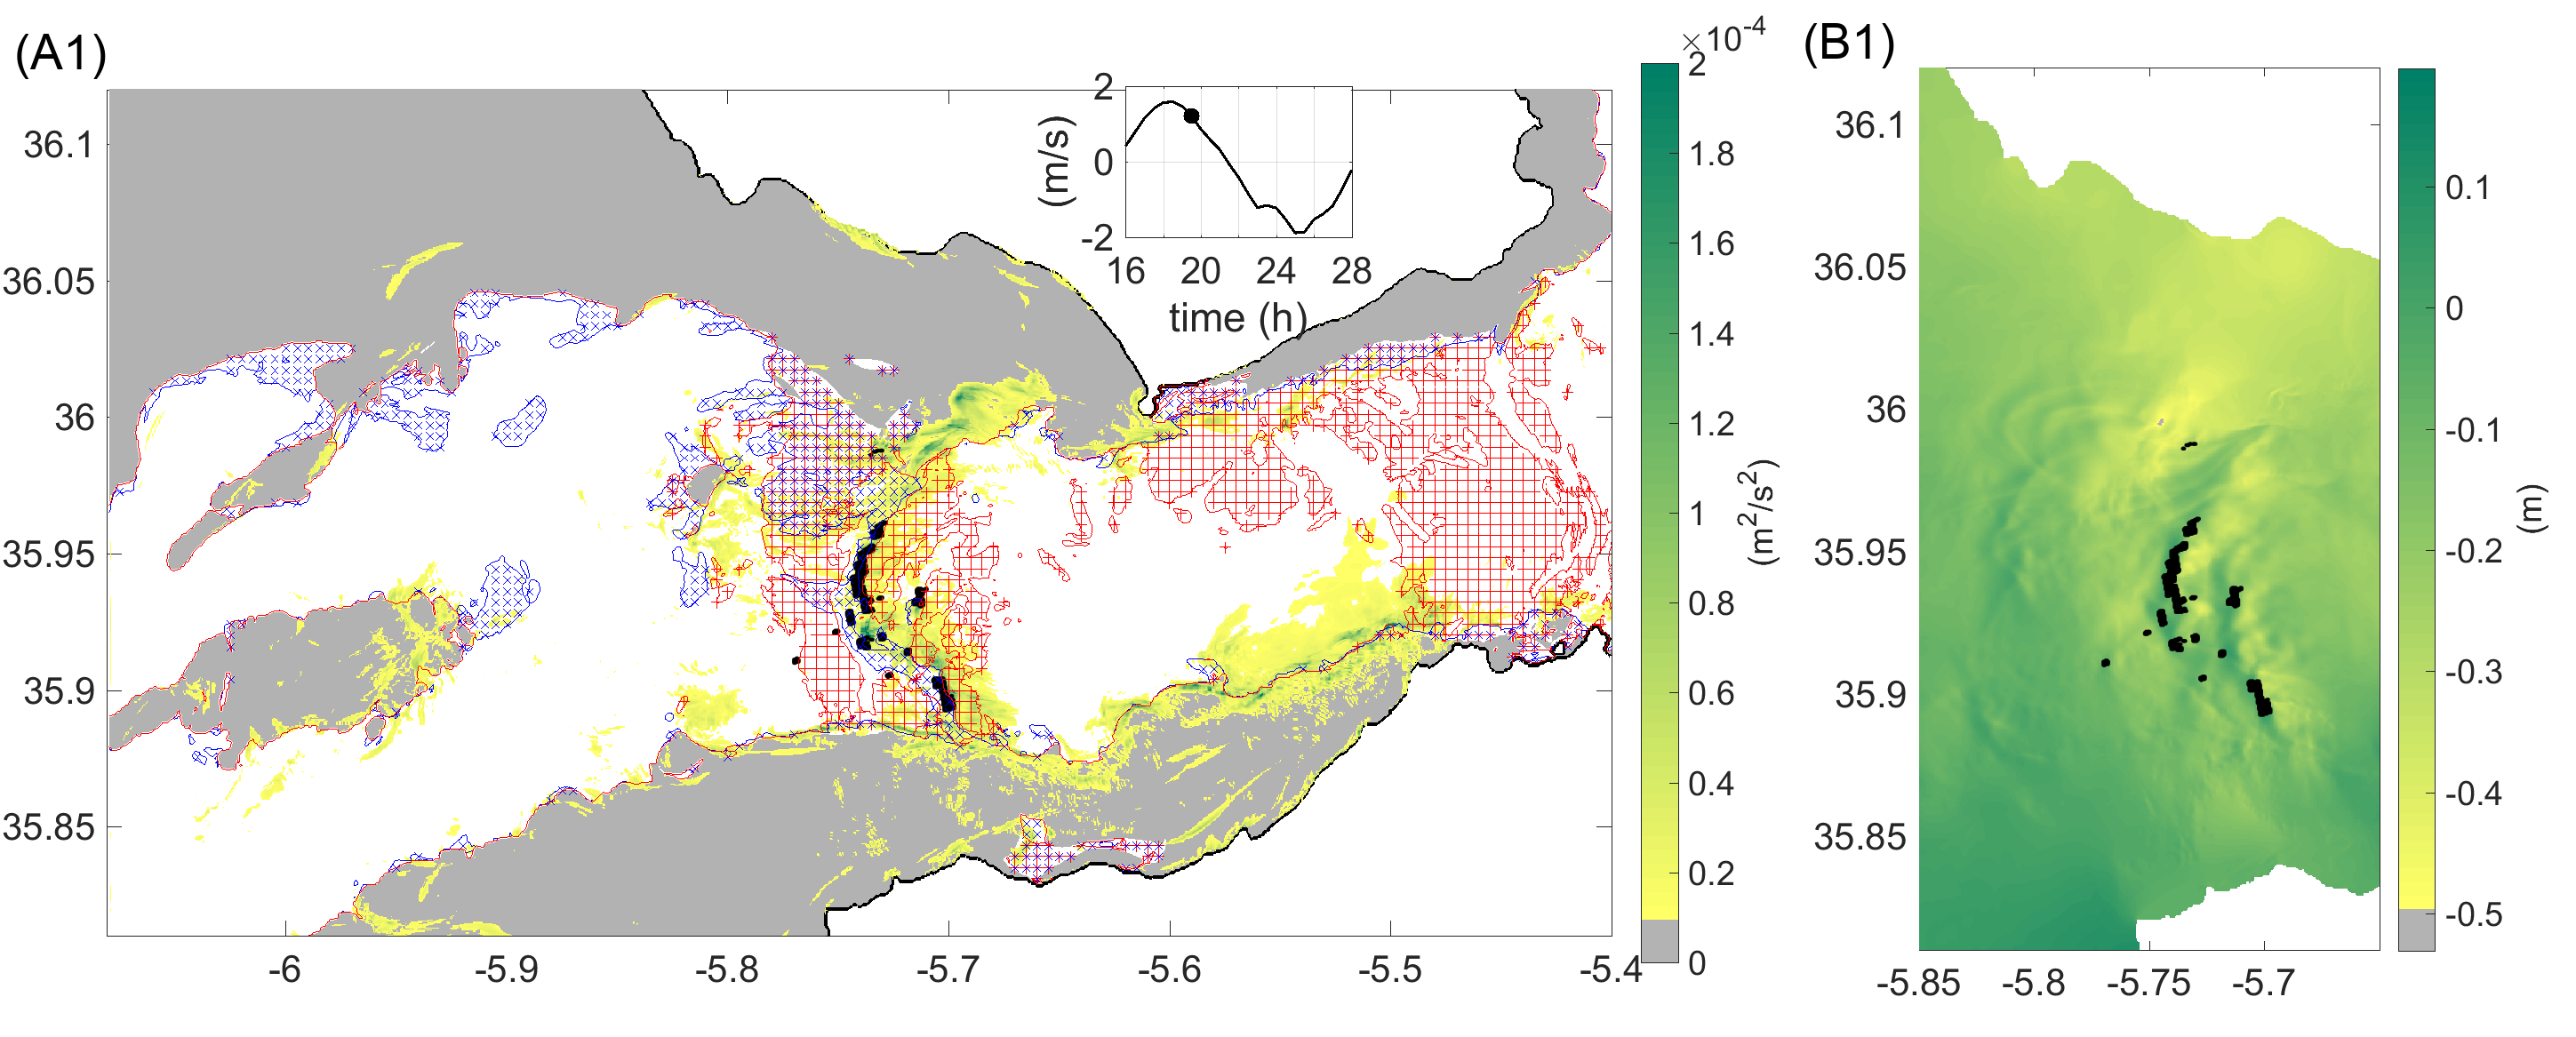
\includegraphics[width=\linewidth]{./GBR3D/VE2_19h30_p.png}
\end{subfigure}

\begin{subfigure}{\linewidth}
\centering
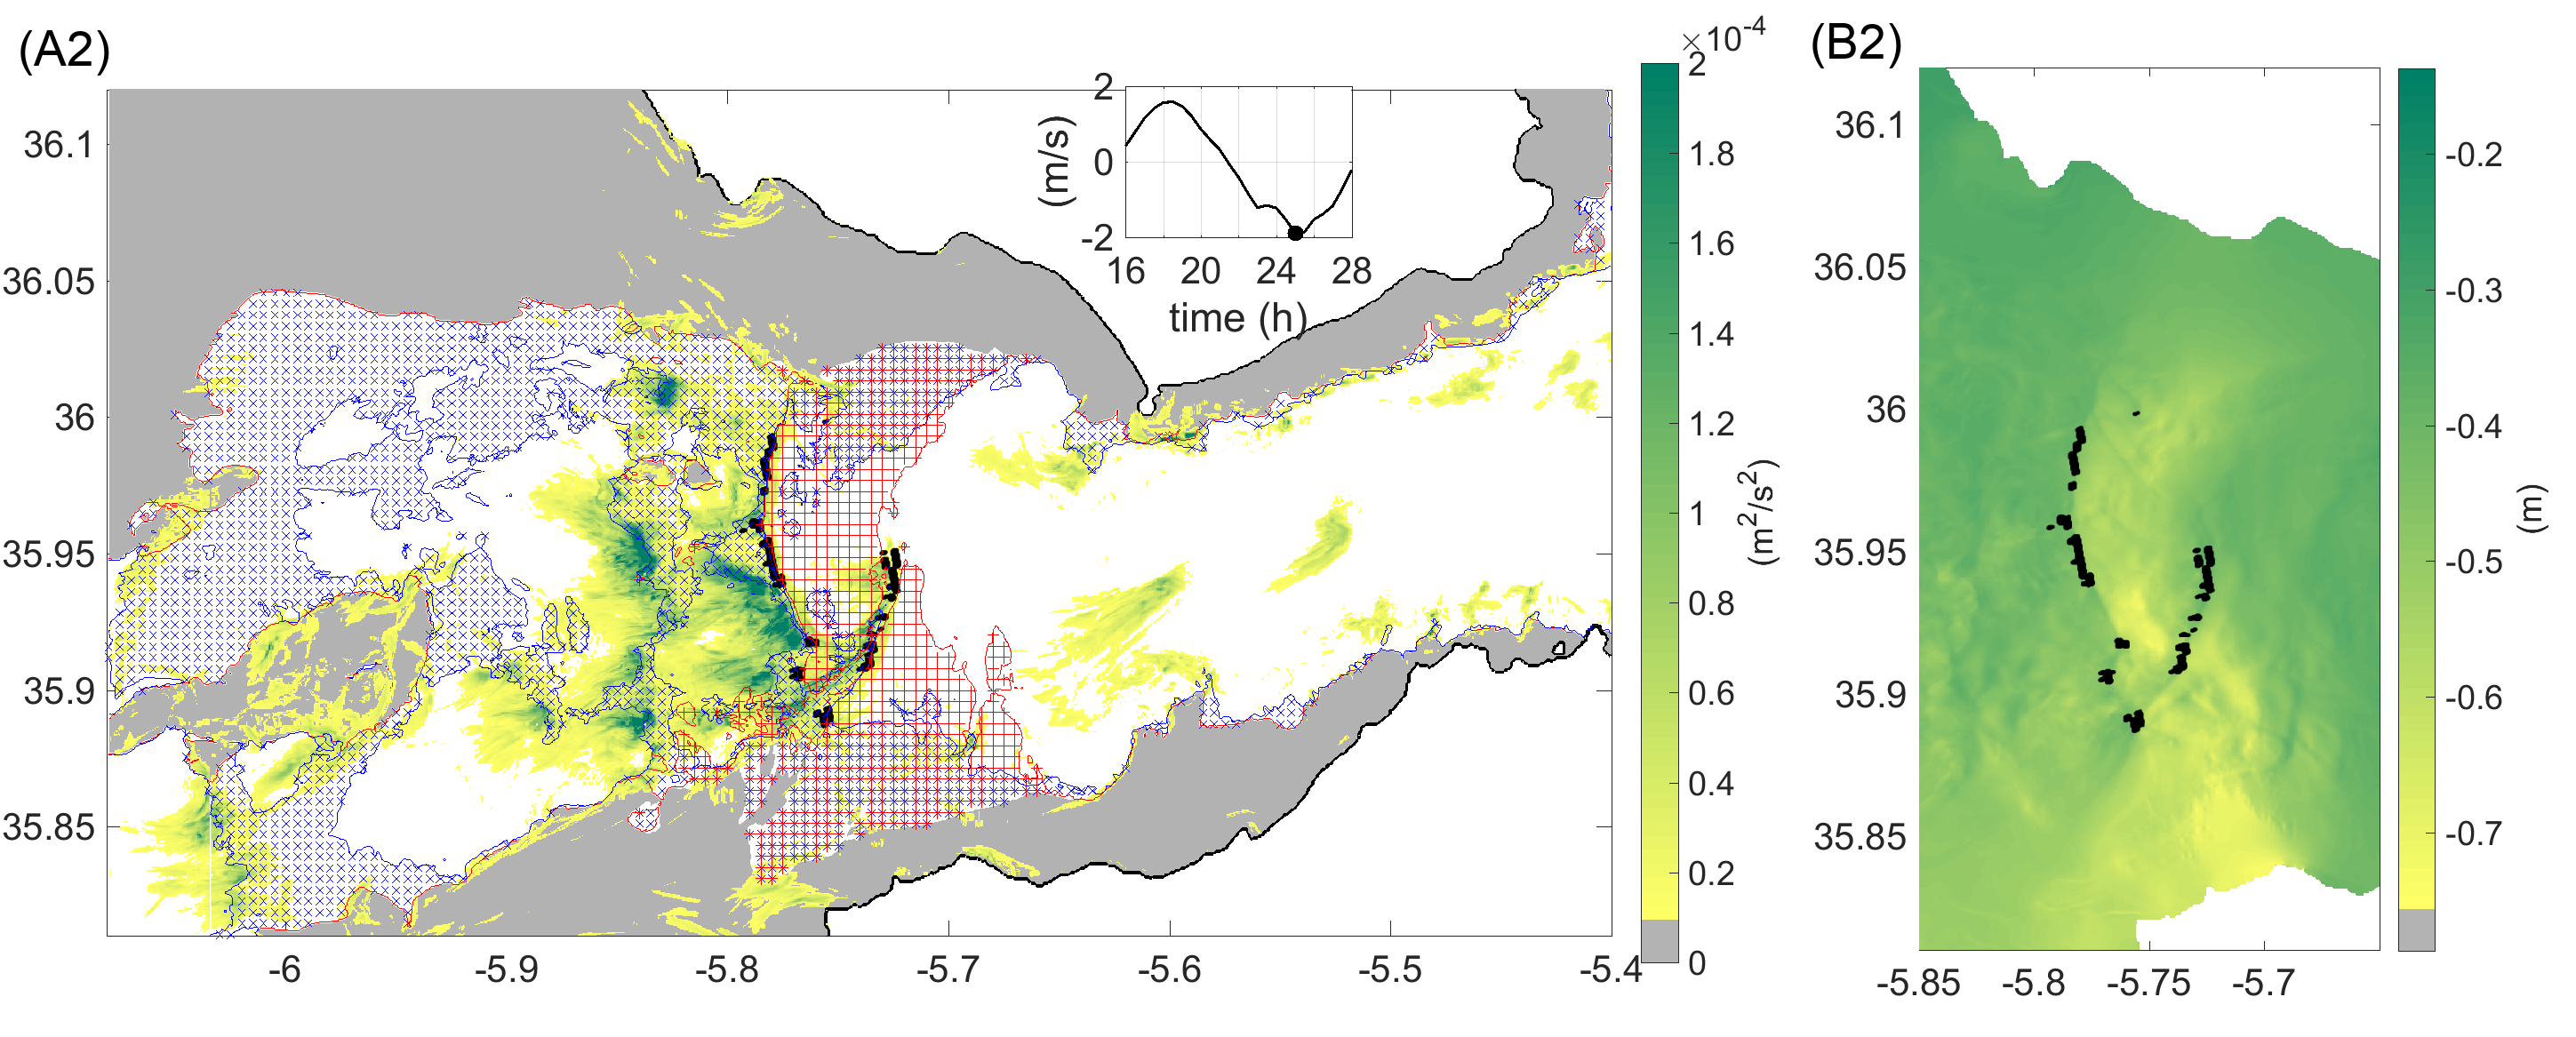
\includegraphics[width=\linewidth]{./GBR3D/VE2_25h_p.png}
\end{subfigure}
\caption {Same as figure \ref{FigHCN} for simulation SimST in inflow and outflow of type \textit{w-jump}}
\label{FigHCS}
\end{figure}

\begin{figure}[!h]
 \centering
%\begin{subfigure}{\linewidth}
%\centering
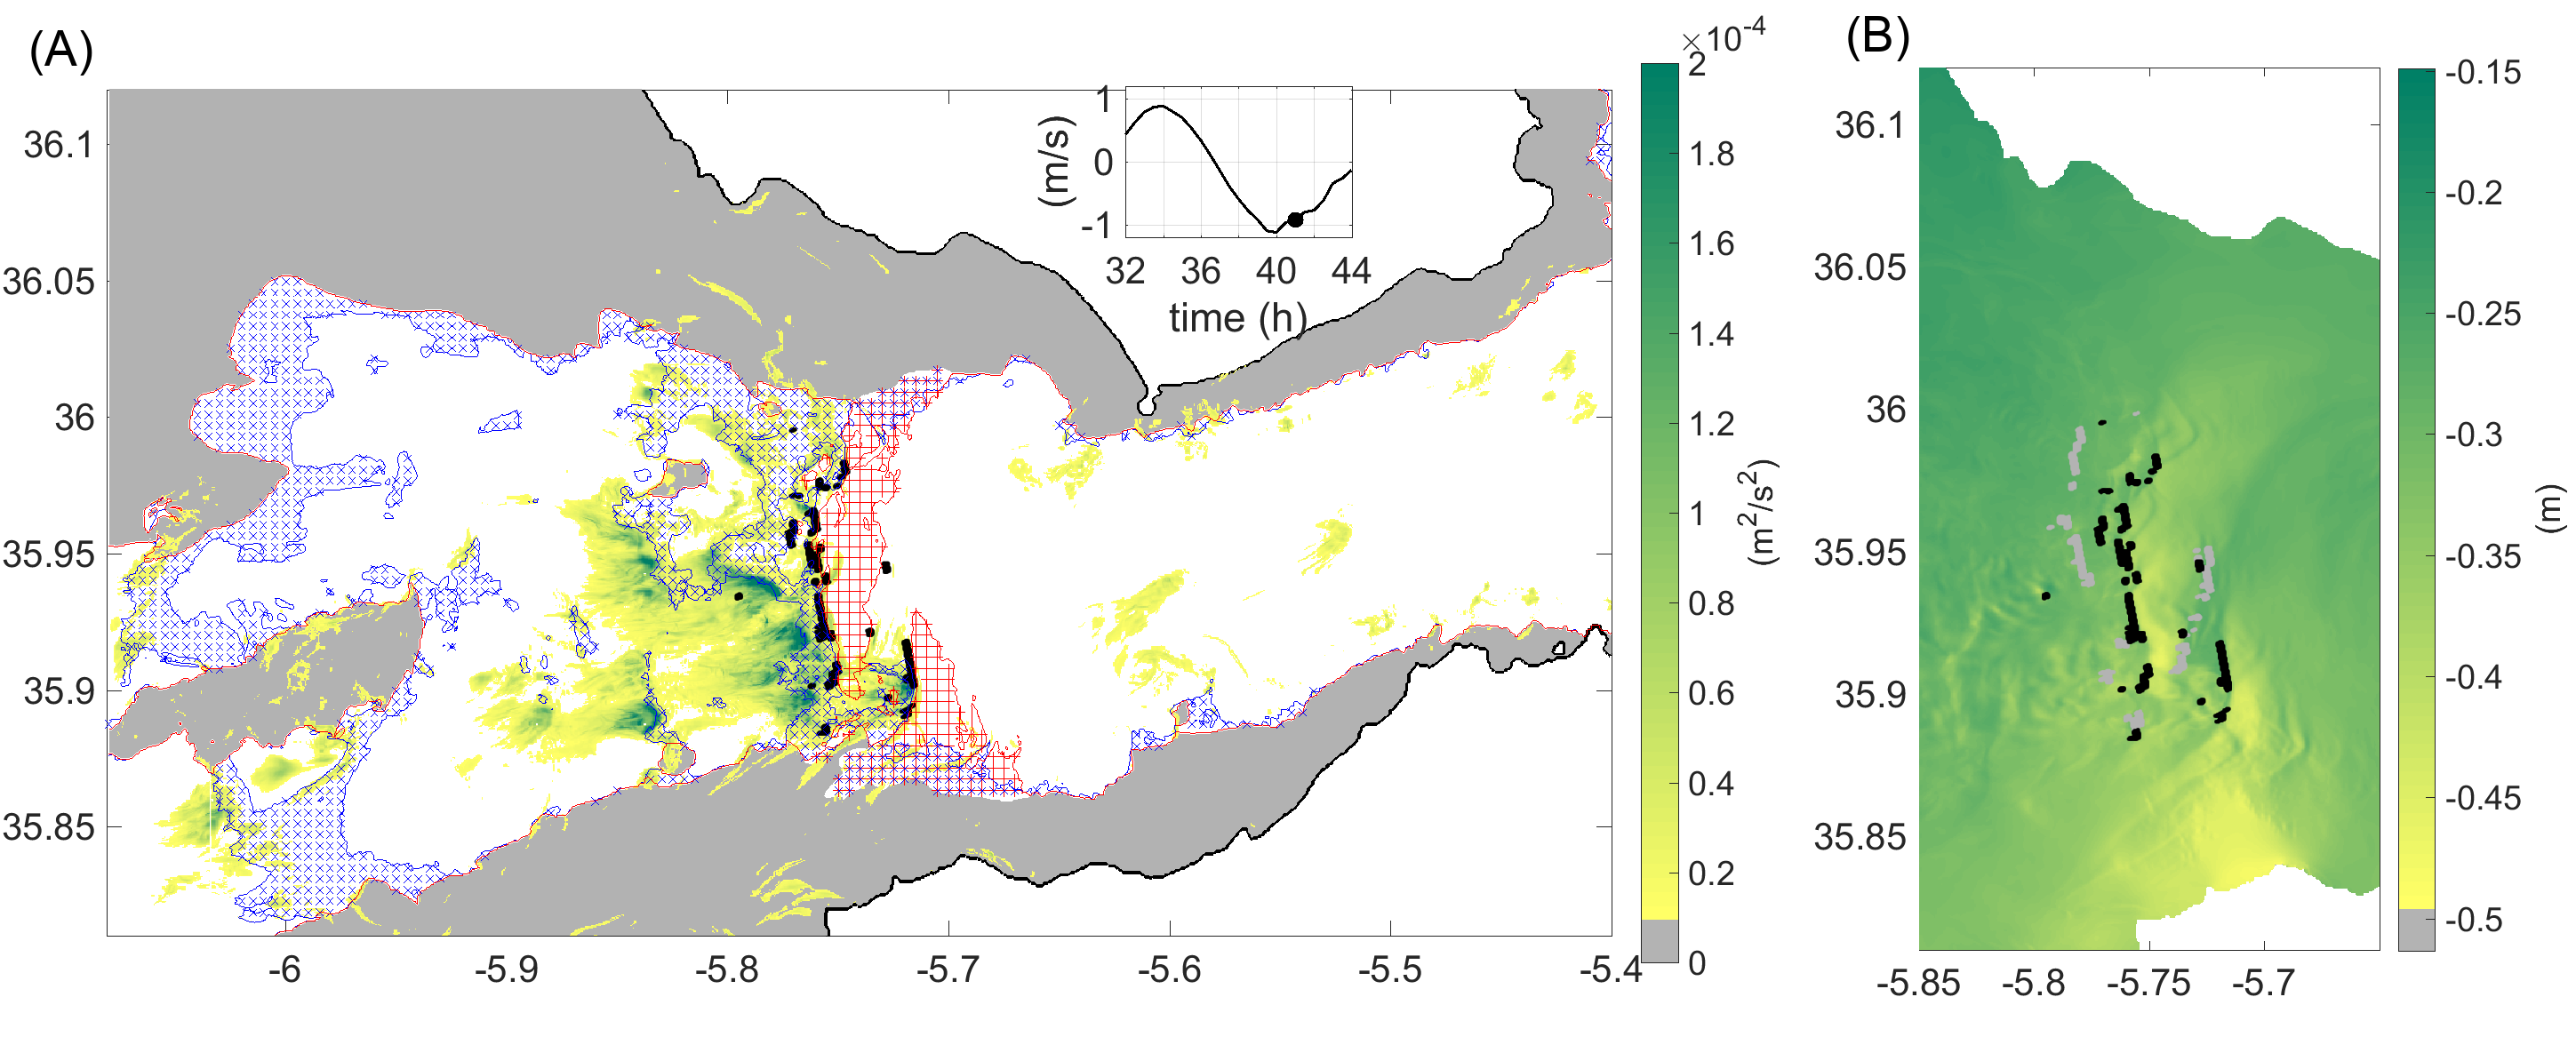
\includegraphics[width=\linewidth]{./GBR3D/IES_41h_p.png}
%\end{subfigure}
 \caption {Same as figure  \ref{FigHCN} for simulation SimIT and an outflow of type {s-jump}, on figure SLA also put trace of jump of spring tide outflow}
 \label{FigHCI}
\end{figure}

\color{green}Attention, tu as laissé beaucoup de formulations sans verbe de ce type: 
\sout{Firstly, can see two channels west of the Camarinal Sill where Med layer is present, separated by Majuan Bank.} ???\color{black}
\color{blue}Firstly, two veins of Mediterranean water separated by Majuan ban can be found west of Camarinal sill.
The southern vein does not change much, however in the northern channel see a variable area of circulation for med waters above 200m depth and centered at 36$^\text{o}$ N. \color{green}Reformule lorsque pas de sujet... la tournure me semble peu usuelle en anglais ? Une proposition suit:\\
 \color{blue}
The southern vein does not change much, however in the northern channel, a variable  \color{green} What do you mean by variable ? Inhomogeneous ? \color{blue} area of circulation of Mediterranean water can be found above a depth of 200 m, this veine is centered at 36$^\text{o}$ N.  \color{black}

This area is larger during outflows, as Mediterranean waters are driven up-slope by the westward barotropic current, but \color{blue} the flow also presents a \color{black}  southern component that bends back into the main north channel (see figure \ref{FigBathy3D} for a better view of the bathymetry of the area).

For all cases, \color{blue} supercritical areas \color{black}  of the Atlantic (Mediterranean) layer \color{blue} can be found \color{black} mostly east (west) of 5.8 $^\text{o}$W which is the western slope of Camarinal sill. During inflows in figure  \color{blue}(\noparref{FigHCN}.a) and (\noparref{FigHCS}.a), the Mediterranean layer becomes supercritical over patches, the most extended one in the area of the northern channel has been discussed above. In outflows in Figures (\noparref{FigHCN}.b), (\noparref{FigHCS}.b) \color{green} Je t'ai reformulé qq citations du type 4.a, je te laisse les éventuelles suivantes que je n'aurais par trouvées...) \color{black} and \ref{FigHCI} the Mediterranean layer is supercritical at both Camarinal, Espartel Sill and in the northern channel for all cases.  \color{blue}During the spring tide outflow period, most of the northern channel presents a supercritical flow while over Espartel sill there is not much difference between the intermediate and spring tide outflow periods \color{black}.

\color{blue}During the outflow period, the Atlantic layer is supercritical only at CS, except during the neap tide period. When both the Mediterranean and Atlantic layers are supercritical at CS, an hydraulic jump is detected. It is located at the intersection of areas where Atlantic and Mediterranean layers are supercritical. This configuration leads to an area of high gradients of free-surface elevation displacement. Among simulated tidal cycles, three types of flows can be encountered at CS during the outflow period: (i) no hydraulic located just above the sill (figure \noparref{FigHCI}, \textit{s-jump}), and (iii) one hydraulic jump located over the western slope of CS (figure \noparref{FigHCS}.b, \textit{w-jump}). In this latter case, the hydraulic jump actually develops \color{black} over the sill's crest as in the s-jump case but as the tidal currents strengthen, \color{blue} an area of supercritical flow develops in the western part of the Atlantic layer and so does the junction where an hydraulic jump can be observed.\color{black} 

\color{blue}An hydraulic jump appears also during inflows, it remains in the same area over the east slope of CS regardless of the strength of tidal currents. It is more pronounced when barotropic currents are stronger, during the transition of flow just upstream of the area of supercritical Atlantic layer. \color{black}

East of CS, another area of supercritical Atlantic layer appears during inflows.  \color{blue}During neap-tide, \color{black} it takes the appearance of a patch near north shore in TN at 5.59$^o$W. During spring tide, this patch extends over a larger area. A secondary area of supercritical Atlantic flow exists between 5.5$^o$W and 5.4$^o$W, extending from the north to the south side of TN. \color{black} 

Figure \ref{FigISWGBR3D} shows \color{blue} the divergence of surface currents in Tarifa Narrows while a train of ISW is propagating. Figure \noparref{FigISWGBR3D}.a corresponds to a barotropic current of intermediate strength during inflow and figure \noparref{FigISWGBR3D}.b to a strong barotropic current during the same period (like figure \ref{FigHCS}.b). \color{black} Are also shown the areas of critical Atlantic layer flow as a black meshed area. The propagation of the ISW train occurs \color{blue} during the same period with the maximum inflow in this area and the area of critical Atlantic layer is located \color{black} west of the propagating wave train. It seems that the northern part of the critical area of the Atlantic layer is dissociated from its southern part. The former occurs more often and its extension varies while the latter may be modified by the arrival of the ISW. This can be due either to induced velocity or to the change of stratification. \color{black}



\begin{figure}[!h]
 \centering
%\begin{subfigure}{\linewidth}
%\centering
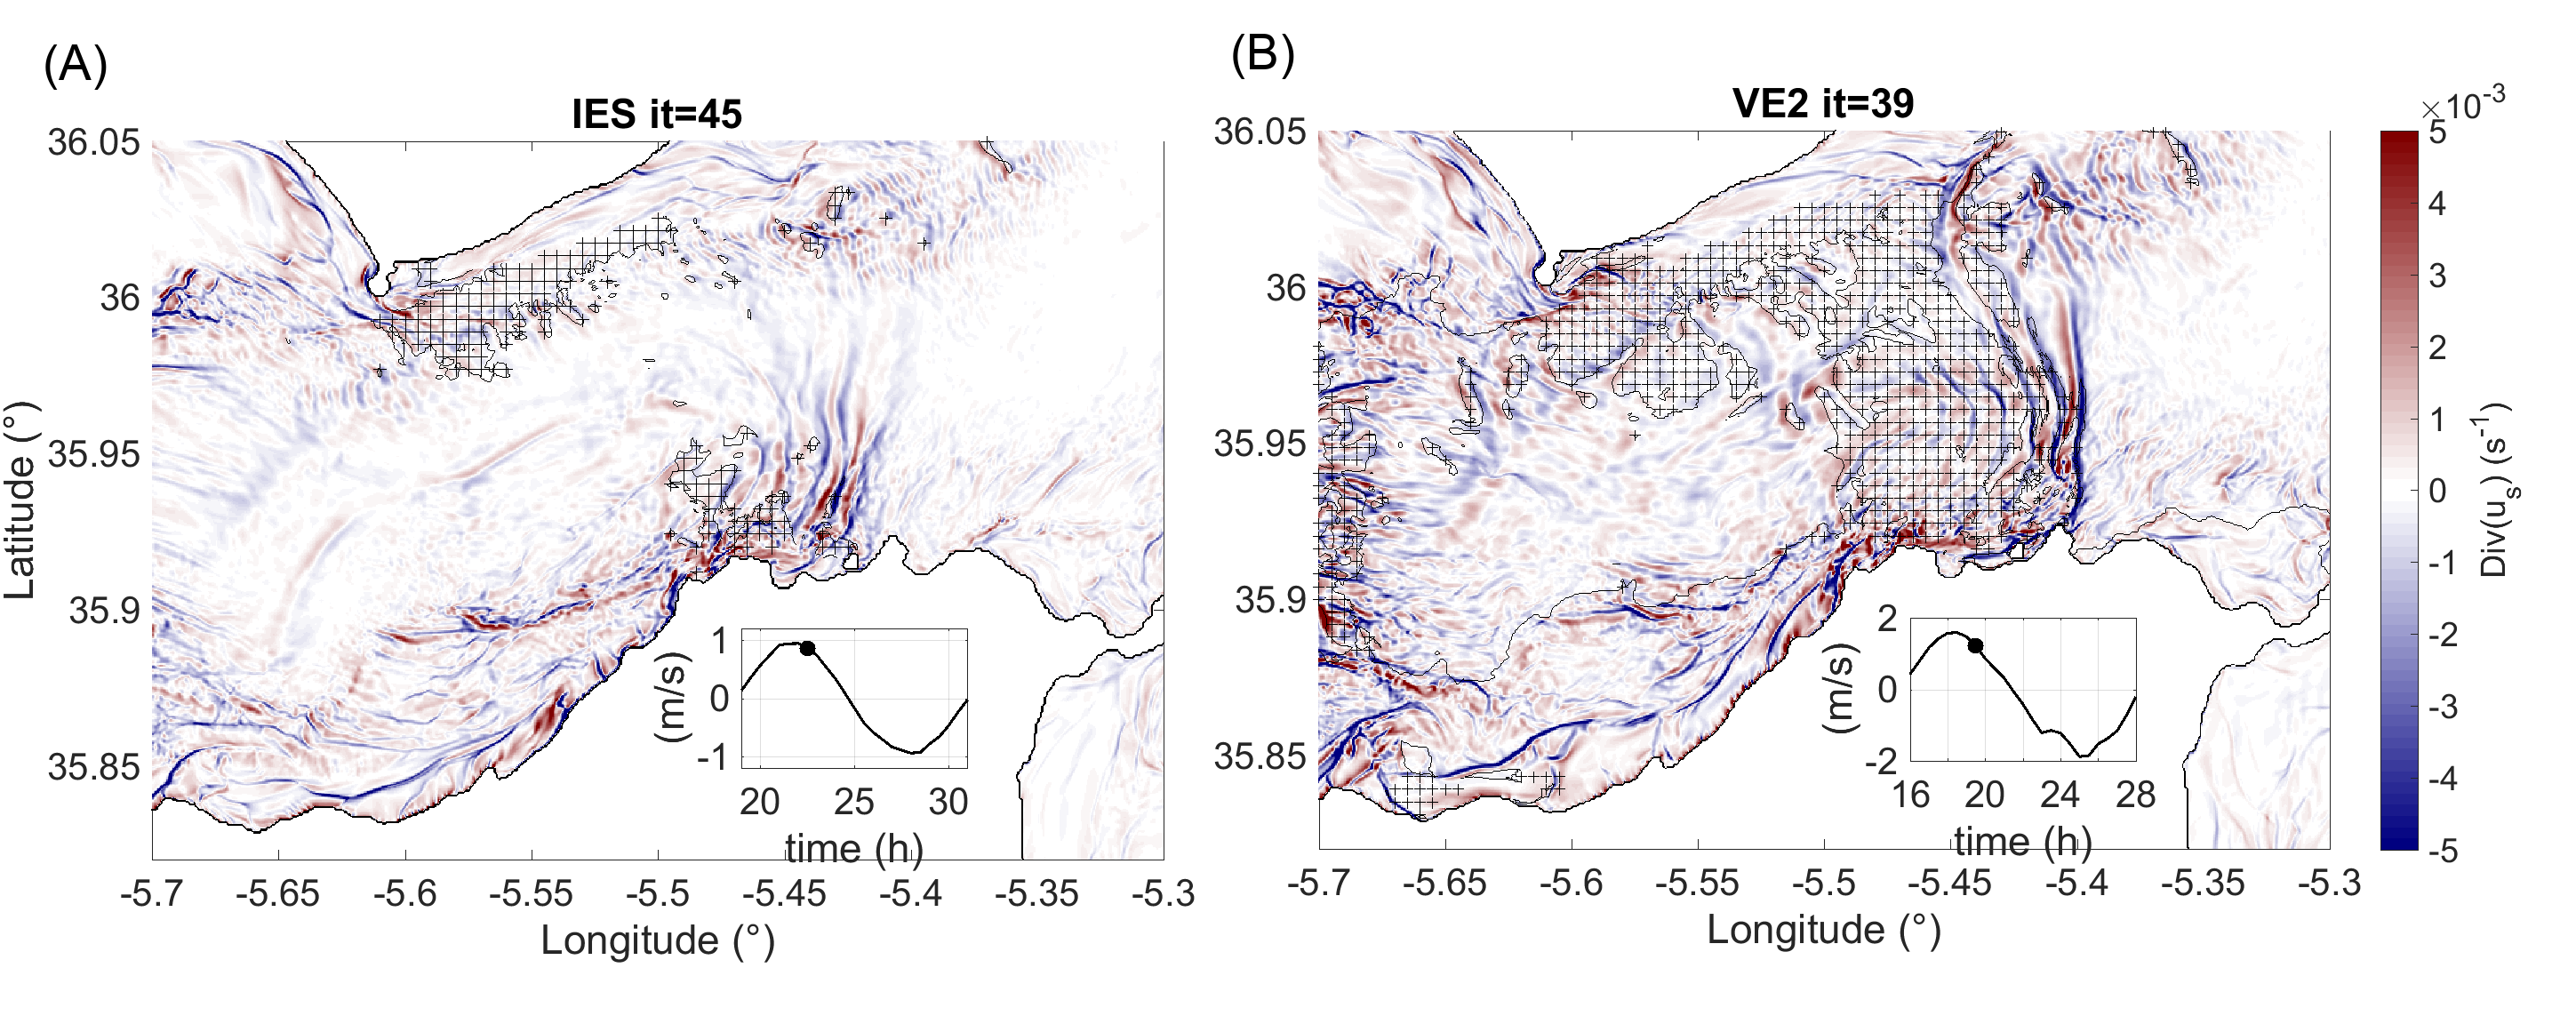
\includegraphics[width=\linewidth]{./GBR3D/FigWaveCont.png}
%\end{subfigure}
 \caption {Divergence of surface current (color) and areas of supercritical atlantic layer (black hatchs) at t = 22.5 h in SimIT (a) and t = 19.5 h in SimST (b)}
 \label{FigISWGBR3D}
\end{figure}

\subsection{Propagation of Solitons (ISWs)}

\begin{figure}[!h]
 \centering
 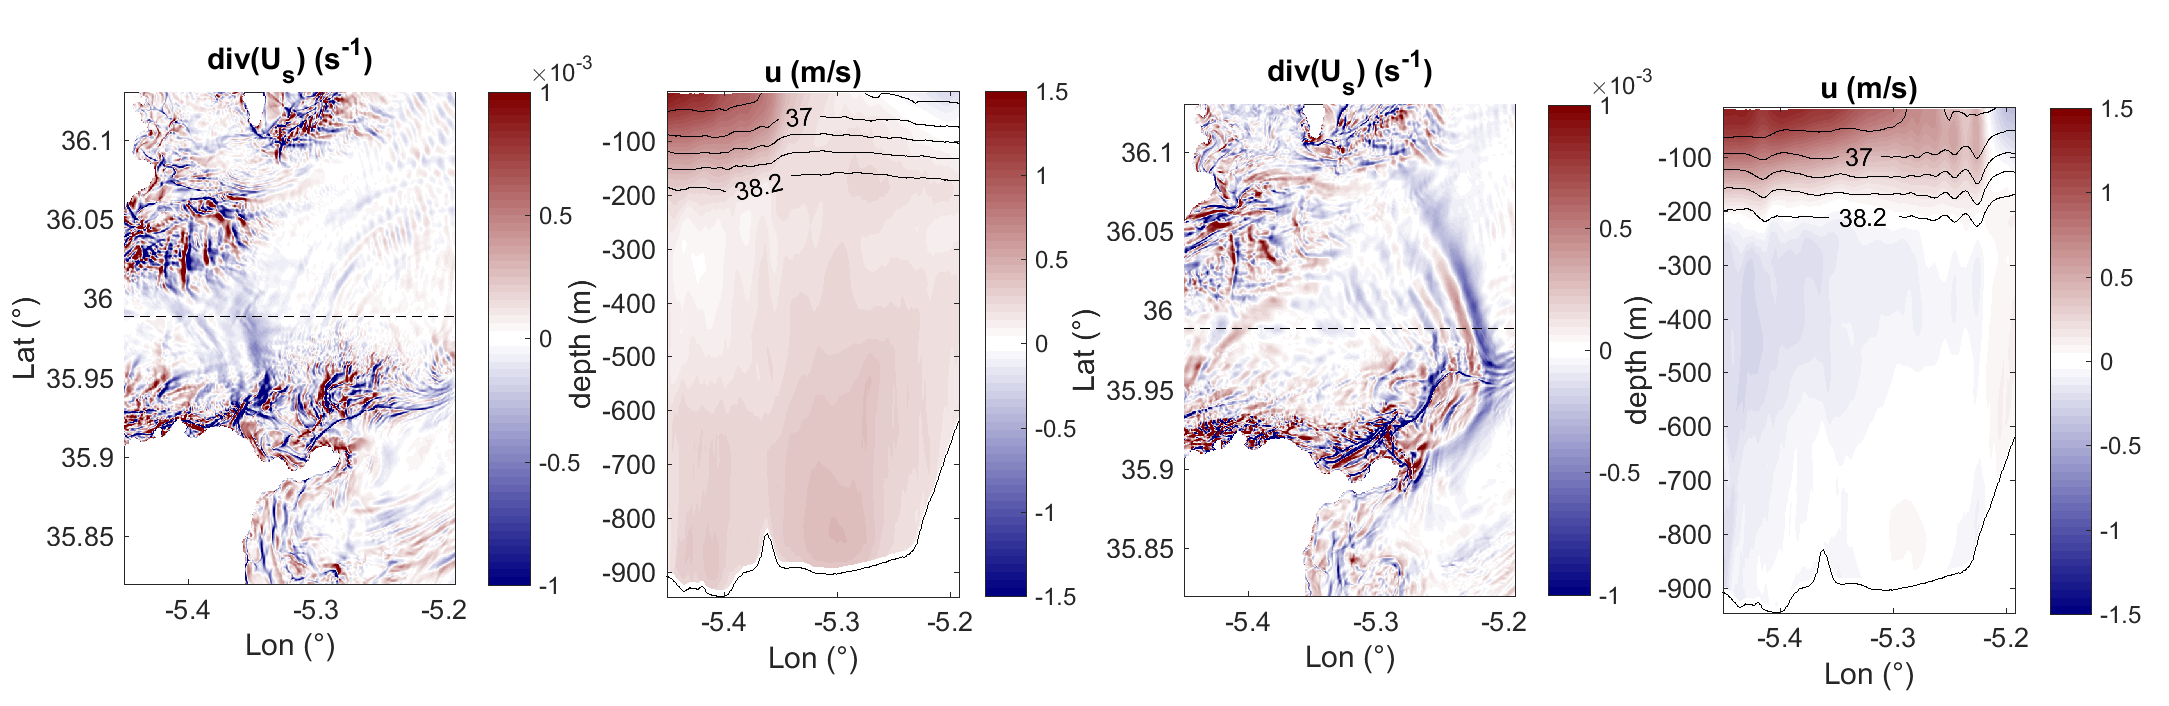
\includegraphics[width=1.\textwidth]{./GBR3D/coupesISW_ME2-2.png}
 \caption {Divergence of surface current (a,c) and vertical section (b,d) of salinity (black ishalines) and zonal velocity $u$ (color) in SimNT at t = 20 h (a,b) and 22 h (c,d) of simulation.}
  \label{FigISWNT}
\end{figure}



\begin{figure}[!h]
 \centering
%\begin{subfigure}{\linewidth}
%\centering
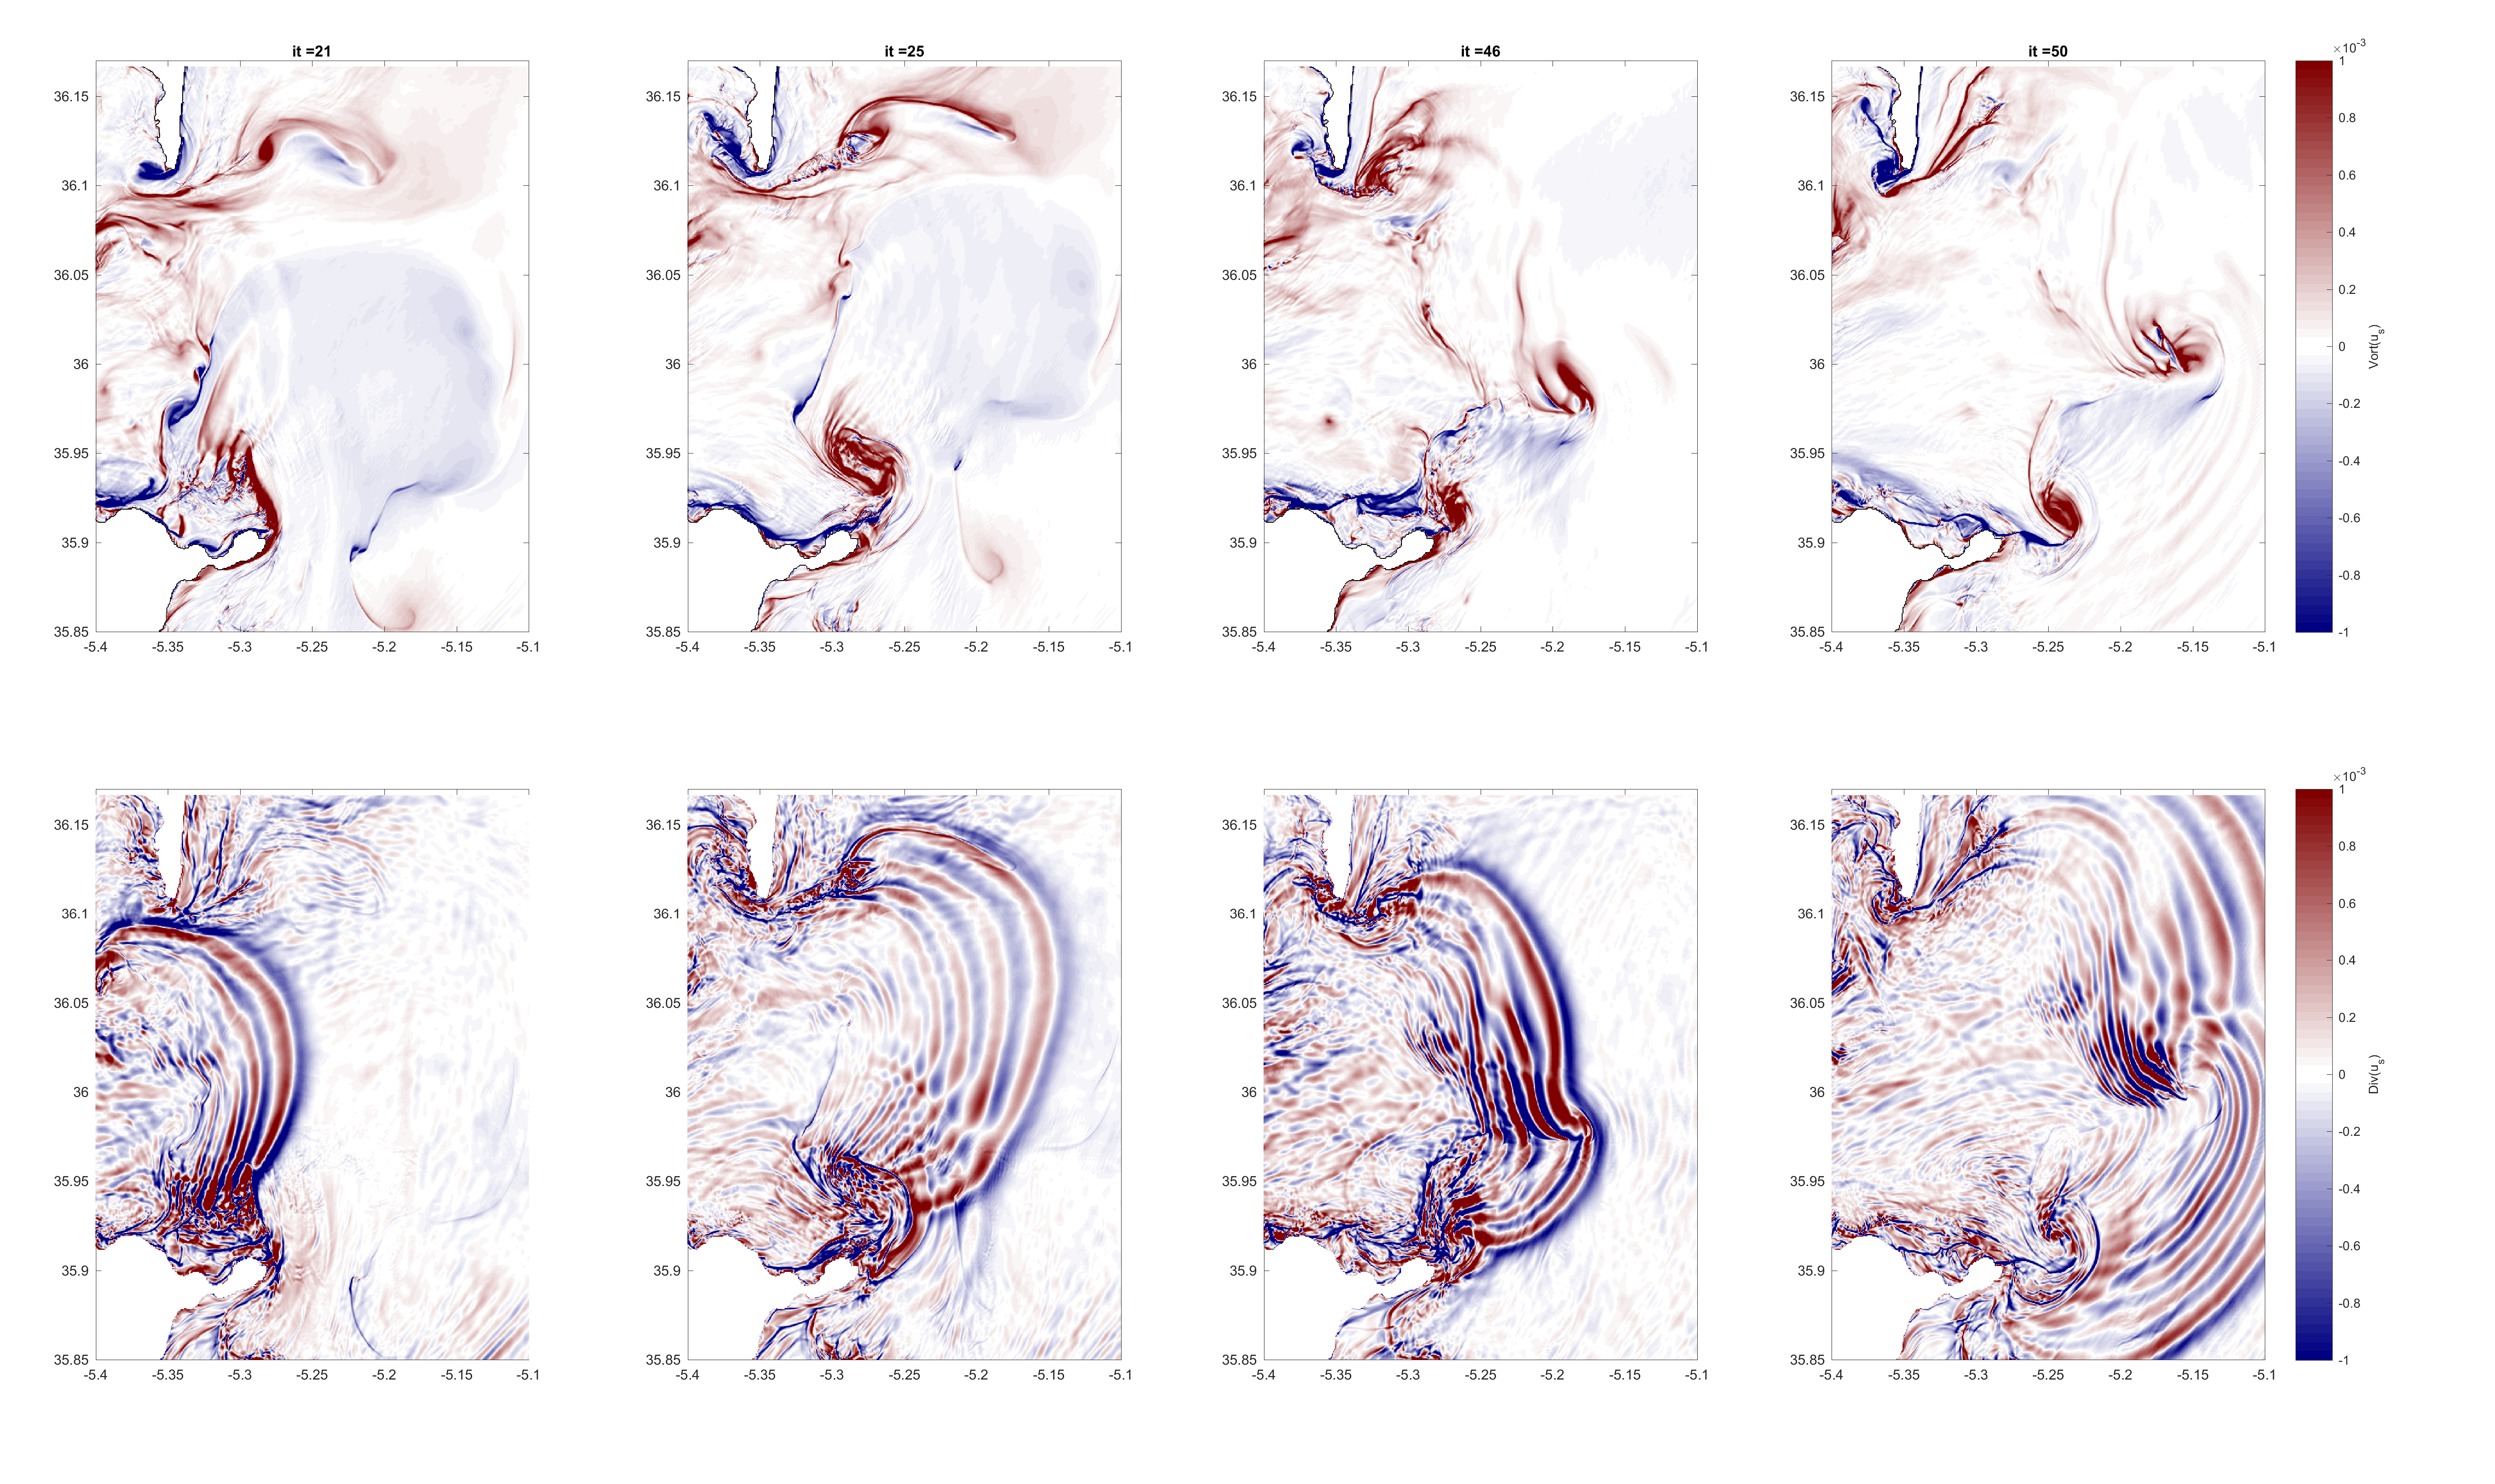
\includegraphics[width=\linewidth]{./GBR3D/FigTourbVE2.png}
%\end{subfigure}
 \caption {Divergence of surface current (upper row) at t = 10.5 h, 12.5 h, then 23 h and 25 h of simulation SimST, and z-axis vorticity of surface current (lower row) for the same time.}
 \label{FigeddGBR3D}
\end{figure}

Solitary waves are observed  \color{blue}after the relaxation of the hydraulic jump at CS (figure \noparref{FigISWGBR3D}). Figures \noparref{FigISWNT}.a and\noparref{FigISWNT}.c also depict the divergence of surface currents but at the eastern exit of the Strait during the \color{black} inflow following a no-jump outflow. Figures \noparref{FigISWNT}.b and \noparref{FigISWNT}.d are vertical sections of the zonal current and salinity at the same time. A train of solitary waves can be observed, this train ends up propagating in the Alboran Sea. Meanwhile, the propagation of the baroclinic tide in figure \noparref{FigISWNT}.b creates a growing front \color{black} with isohalines steepening due to non-linear effects. As is the case for the ISW generated at CS, non-hydrostatic dispersion balances this effect to create a train of solitary waves. In SimNT this process occurs following all \textit{no-jump} outflows.

\color{blue}However, compared to the upper row of figure \ref{FigeddGBR3D} (also showing the divergence of surface currents during the tidal periods following the hydraulic jump at CS), the train of solitary waves observed in the Alboran Sea after a \textit{no-jump} outflow is less extended and presents fewer solitons.  \color{black}

Figures (\noparref{FigeddGBR3D}.a-b) then (\noparref{FigeddGBR3D}.a-d) show two inflow periods separated by one tidal cycle in SimST configuration. The lower row of \color{blue} figure \ref{FigeddGBR3D} exhibits the z-component of the surface vorticity \color{black} at the same time. In the first two figures of each row, a train of solitary waves leaves the strait \color{blue} and enters in the Alboran Sea. The number of solitons in the train increases during this period. \color{black} A filament of positive vorticity is formed by interaction with the south coast in (\noparref{FigeddGBR3D}.e) and develops into a cyclonic eddy in (\noparref{FigeddGBR3D}.f).  \color{blue}In figure (\noparref{FigeddGBR3D}.c) one tidal cycle later the eddy is located at 5.2 $^\text{o}$W and 36 $^\text{o}$N and the new train of solitary waves is refracted by this eddy: its southern part is indeed accelerated whereas its northern part is decelerated by the induced currents. At the same time a vortical structure can be observed in the region of Ceuta. In figure (\noparref{FigeddGBR3D}.d) this structure has also evolved into \color{black} a cyclonic eddy that propagates in the Alboran Sea. Meanwhile the interaction between the solitary waves and the previous cyclonic eddy has resulted into an interference pattern in the wave packet. 


In the simulations, this process of generation of cyclonic eddies \color{blue} in the region of Ceuta \color{black} occurs each time a train of solitary waves exits the strait.  The train of the next tidal cycle gets diffracted on this eddy, creating local \color{blue}modifications of the structure of the train. \color{black}


\subsection{Dynamical structures at Camarinal Sill, primary instabilities}

\subparagraph{Neap-tide cycle}

Along with the features of the flow already discussed previously, figures \ref{FigHCN}, \ref{FigHCS} and \ref{FigHCI} indicate patches of high standard deviation of parameter Q \color{blue} defined in section (XXX). The extension of these patches is maximal during all outflow periods \color{black} and for the spring-tide inflow  \color{green} (you mean "spring-tide flow"?), \color{black} although the values  \color{green}(which values, standard deviations?) \color{black} for this latter case are not as large and the patch itself is not as extended. High values of the \color{blue} standard deviation \color{black} indicate the occurence of large-amplitude oscillations of the values of parameter Q. \color{blue} Larger standard deviations can be found during the two outflow periods during which the hydraulic jump \color{black} is detected (\textit{w-jump} and \textit{s-jump}) west of CS at 5.79 $^\text{o}$W and west of secondary bathymetric features in Tangier basin at 5.84 $^\text{o}$W. There is also \color{blue} a smaller amplitude \color{black} signal at ES, of greater standard deviation for the spring tide outflow \color{green}(not sure to understand what you mean...). \color{black}

\color{blue}Figure (\noparref{FigTSCS}.a) superposes the standard deviation and \color{black} the singular vector of SVD performed on the 3D field of parameter Q computed during the outflow for the EOF that had the most high-frequency variability in its eigenvector, associated with propagation of vortices (the higher order EOFs (not shown) have low frequency variability and structure associated with the regional flow itself). \color{green}(la phrase est longue, longue... Tu peux la découper en phrases très courtes d'une part mais surtout commencer par un petit paragraphe d'explications/introductions sur ta SVD... Pourquoi, comment etc...) \color{black}

As expected, the contours of parameter Q  \color{blue}\sout{$=5e-5m^2s^{-2}$} $5x10^{-5}\ m^2s^{-2}$ plotted the  \color{green}(which?) \color{blue} EOF are co-located with the values of large standard deviation, i.e. on the western slope of CS and the western slope of secondary sills in Tangier Bassin. \color{black} 

\color{blue}Figures (\noparref{FigTSCS}.b) to (\noparref{FigTSCS}.e) show a \color{blue}part \color{black} of $\theta$-S diagram showing  the region of the signature of all the simpulation grid-points at a given longitude zoomed in Mediterranean waters. Figure (\noparref{FigTSCS}.b) shows that at 5.76$^text{o}$ W, still over the crest of the sill, the repartition among Mediterranean waters remains similar to \color{black} the one found in figure \ref{Fig_Ini_WM3D} at the east entry of the strait. \color{blue}Figures (\noparref{FigTSCS}.c) and (\noparref{FigTSCS}.d) present the evolution of this $\theta$-S diagram along the path of what becomes the Mediterranean outflow: \color{black} the water parcels are homogenizing and can be classified into three to four water masses.

These diagrams are \color{blue}more specifically \color{black} plotted for longitudes located in areas of large values of Q, i.e. where mixing processes can be expected. However, clearly, Mediterranean water masses do not homogenize right after after CS.  \color{green}Look into it with (tu n'as pas fini ta phrase???) \color{black}

\begin{figure}[!h]
% \centering
 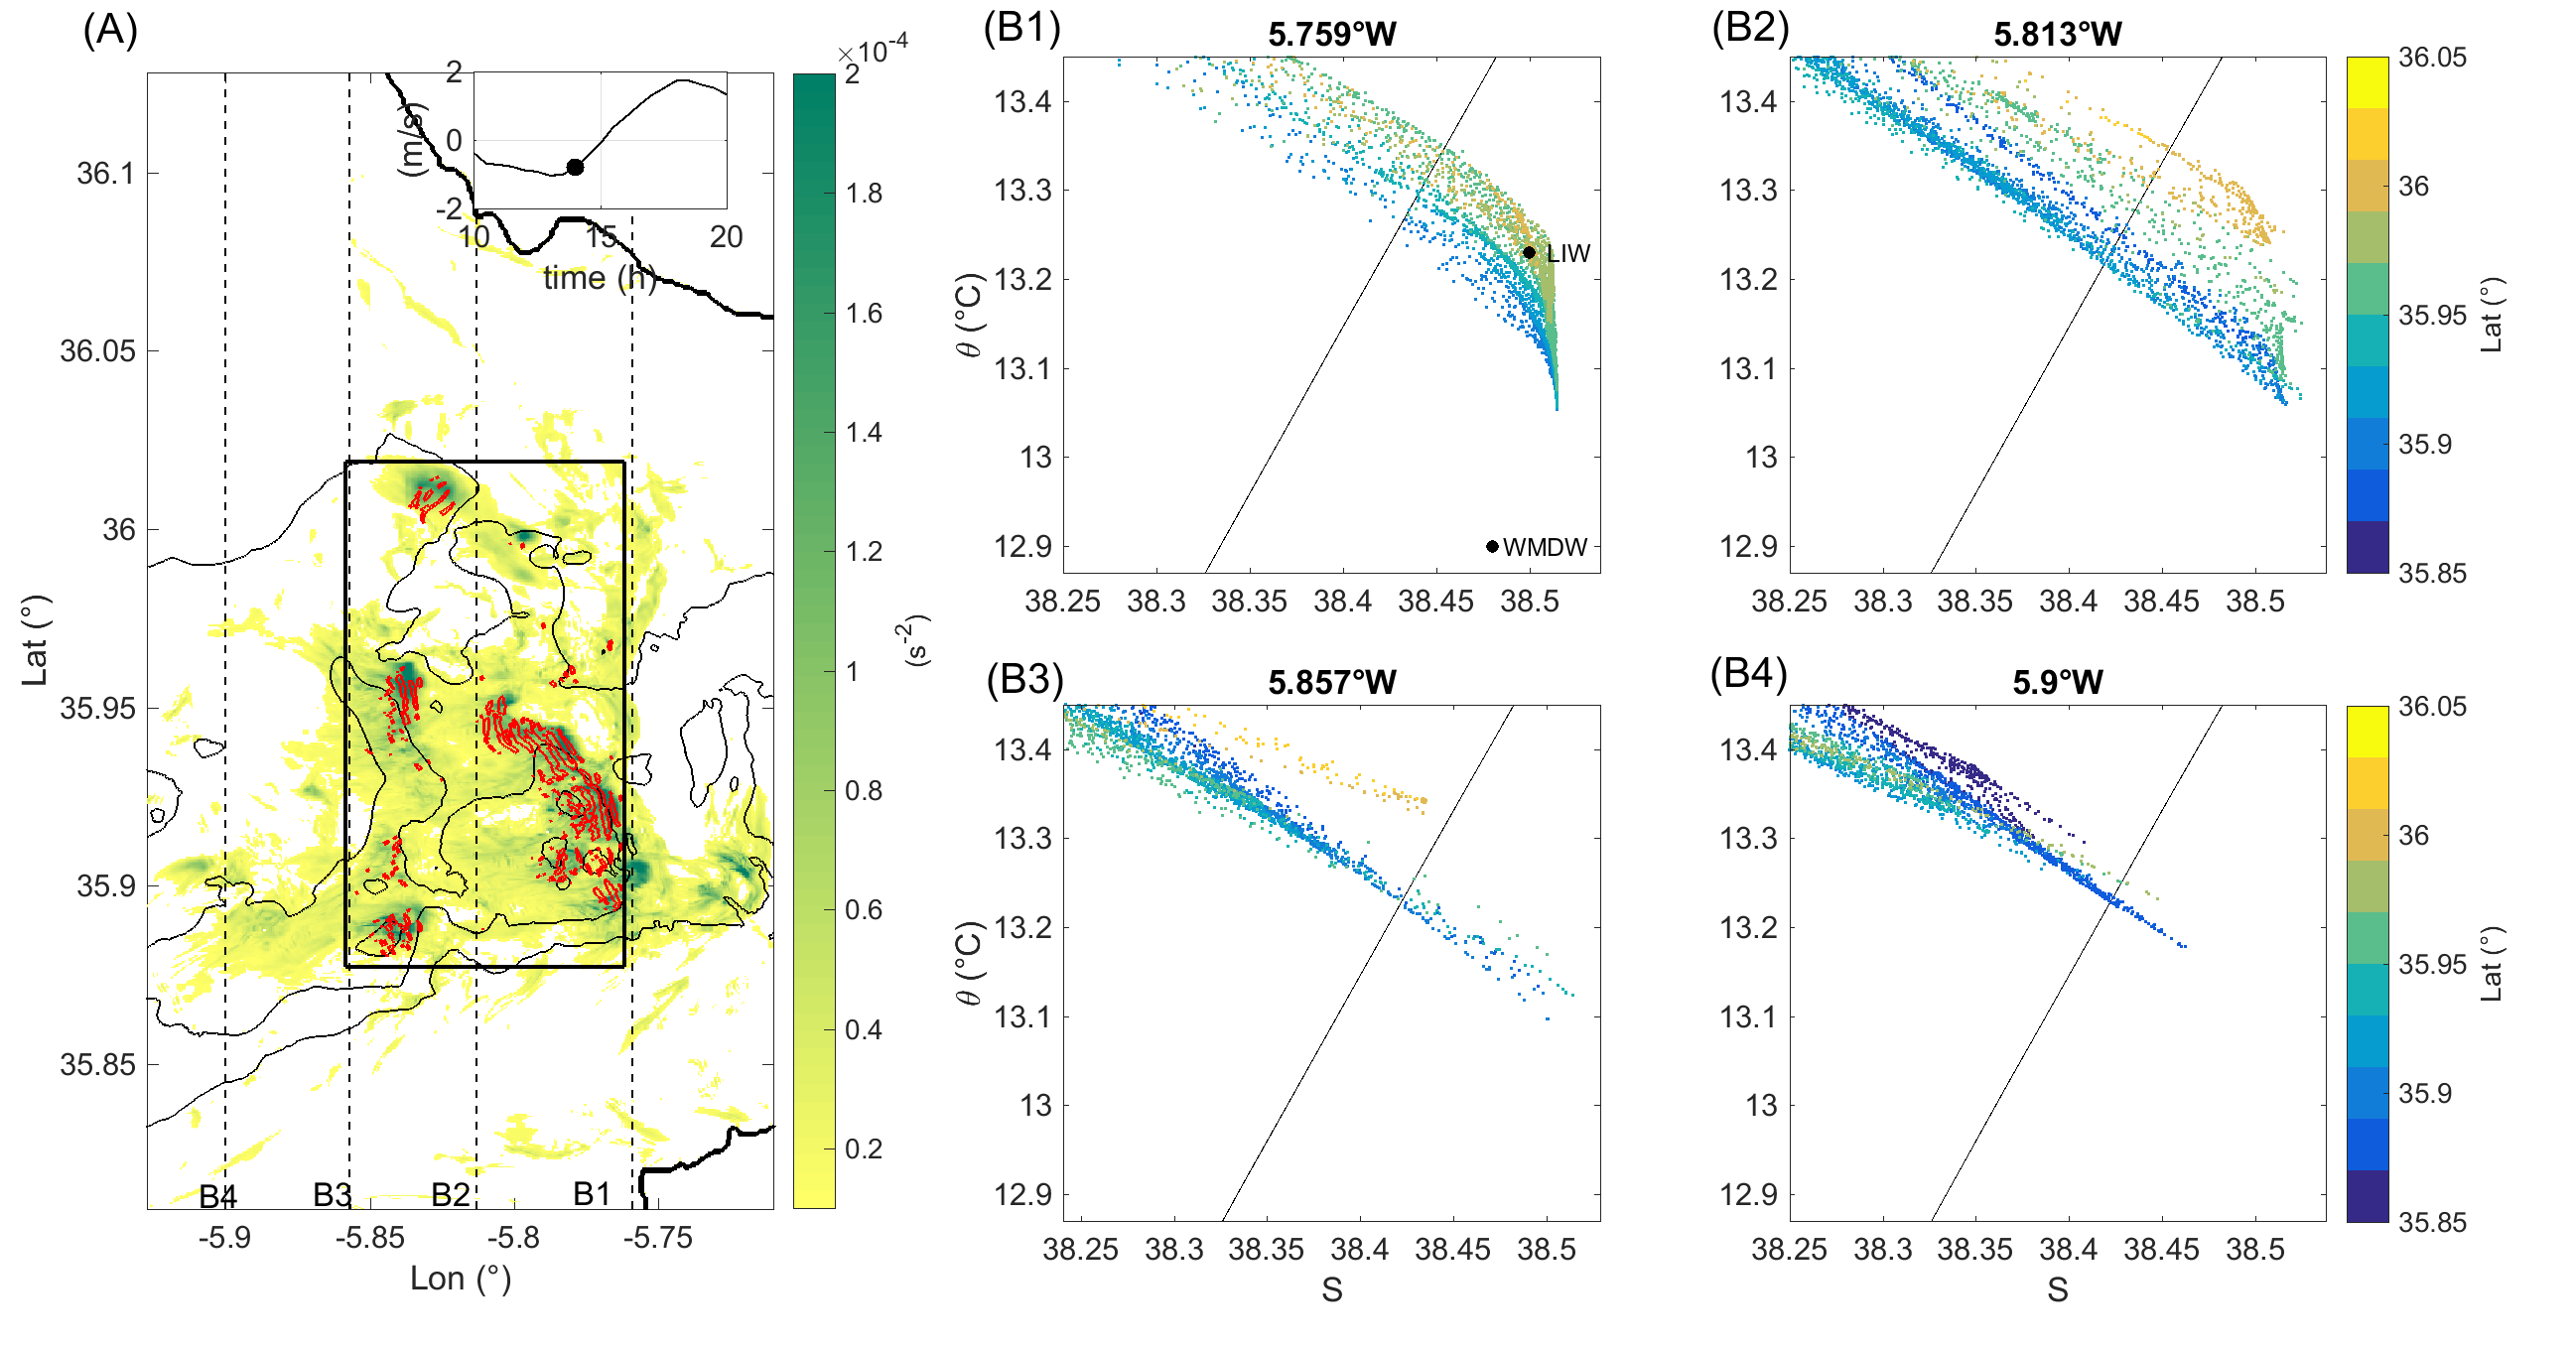
\includegraphics[width=\textwidth]{./GBR3D/TS_coupes_14H_VE2o.png}
 \caption {(a) Standard deviation of parameter Q over 30-mn-periods at $t\ =\ 14\ h$ in SimST (color) and trace \color{green}(what do you mean by trace? Isocontours?) of Q $\ =\ 5$\color{black}  from the high-frequency EOF of SVD performed in the rectangular black box during the outflow period. Black dashed lines indicate the longitude at which $\theta-S$ diagrams are plotted. (b,c,d,e) $\theta-S$ diagrams, zoomed in the area of the Mediterranean water masses.  \color{green}(Mettre LETTRES, rajouer section plus au sud?) \color{black}}
 \label{FigTSCS}
\end{figure}

\color{blue}The singular vectors of SVD are now studied varying the strength of the outflows of barotropic tidal currents. \color{black} Figures (\noparref{FigEOFMIV}.a,b,c) present the EOF of parameter Q for the outflows of figures \ref{FigHCN}, \ref{FigHCS},and \ref{FigHCI}, along with vertical sections of salinity plotted \color{blue}at the same date and time \color{black} as figures (\noparref{FigEOFMIV}d,e,f). These sections are plotted along latitude 35.94$^\text{o}$ N. Figure (\noparref{FigEOFMIV}.g) and (\noparref{FigEOFMIV}.h) are histograms giving the height above seafloor and latitude of the grid points of the EOF for which Q $\geq 5e-5\ m^2/s^2$. On vertical sections, we can see that the positive value of Q parameter are associated with billow structures of salinity that develop in the gravity current along the west slope of the CS. Those structures develop for each outflow case, but the wider distributions of height above sea floor and \sout{visualisation} in the vertical section  \color{blue}indicate that \color{black} the billows \color{blue}\sout{have greater radius} are larger in \color{black} when and where an hydraulic jump is present, catching more interfacial and Atlantic waters into the Mediterranean outflow. At this longitude where the instabilities are still \color{blue}well-developed \color{black}, cores are not yet mixed in the simulation. A quick look at the $\theta$-S diagrams shows \color{blue} that the outflow is still heterogeneous.

The cases \color{blue}of hydraulic jumps \color{black} also differ, while instabilities develop along the same areas in \textit{no-jump} and \textit{s-jump} case, in the w-jump case the hydraulic jump and the start of the gravity current are co-localised at all latitude as seen in the vertical section, which adds a possible area of generation between 35.92$^\text{o}$N and 35.93$^\text{o}$N, down slope of the shallowest point of the sill where the flow of Mediterranean waters is not as strong for s-jump and no-jump cases. \color{green} Difficile de suivre le raisonnement jusqu'au bout dans cette longue phrase. Peux-tu la reformuler un peu et la découper en trois ou quatre phrases très courtes ? \color{black}


\begin{figure}[!h]
% \centering
 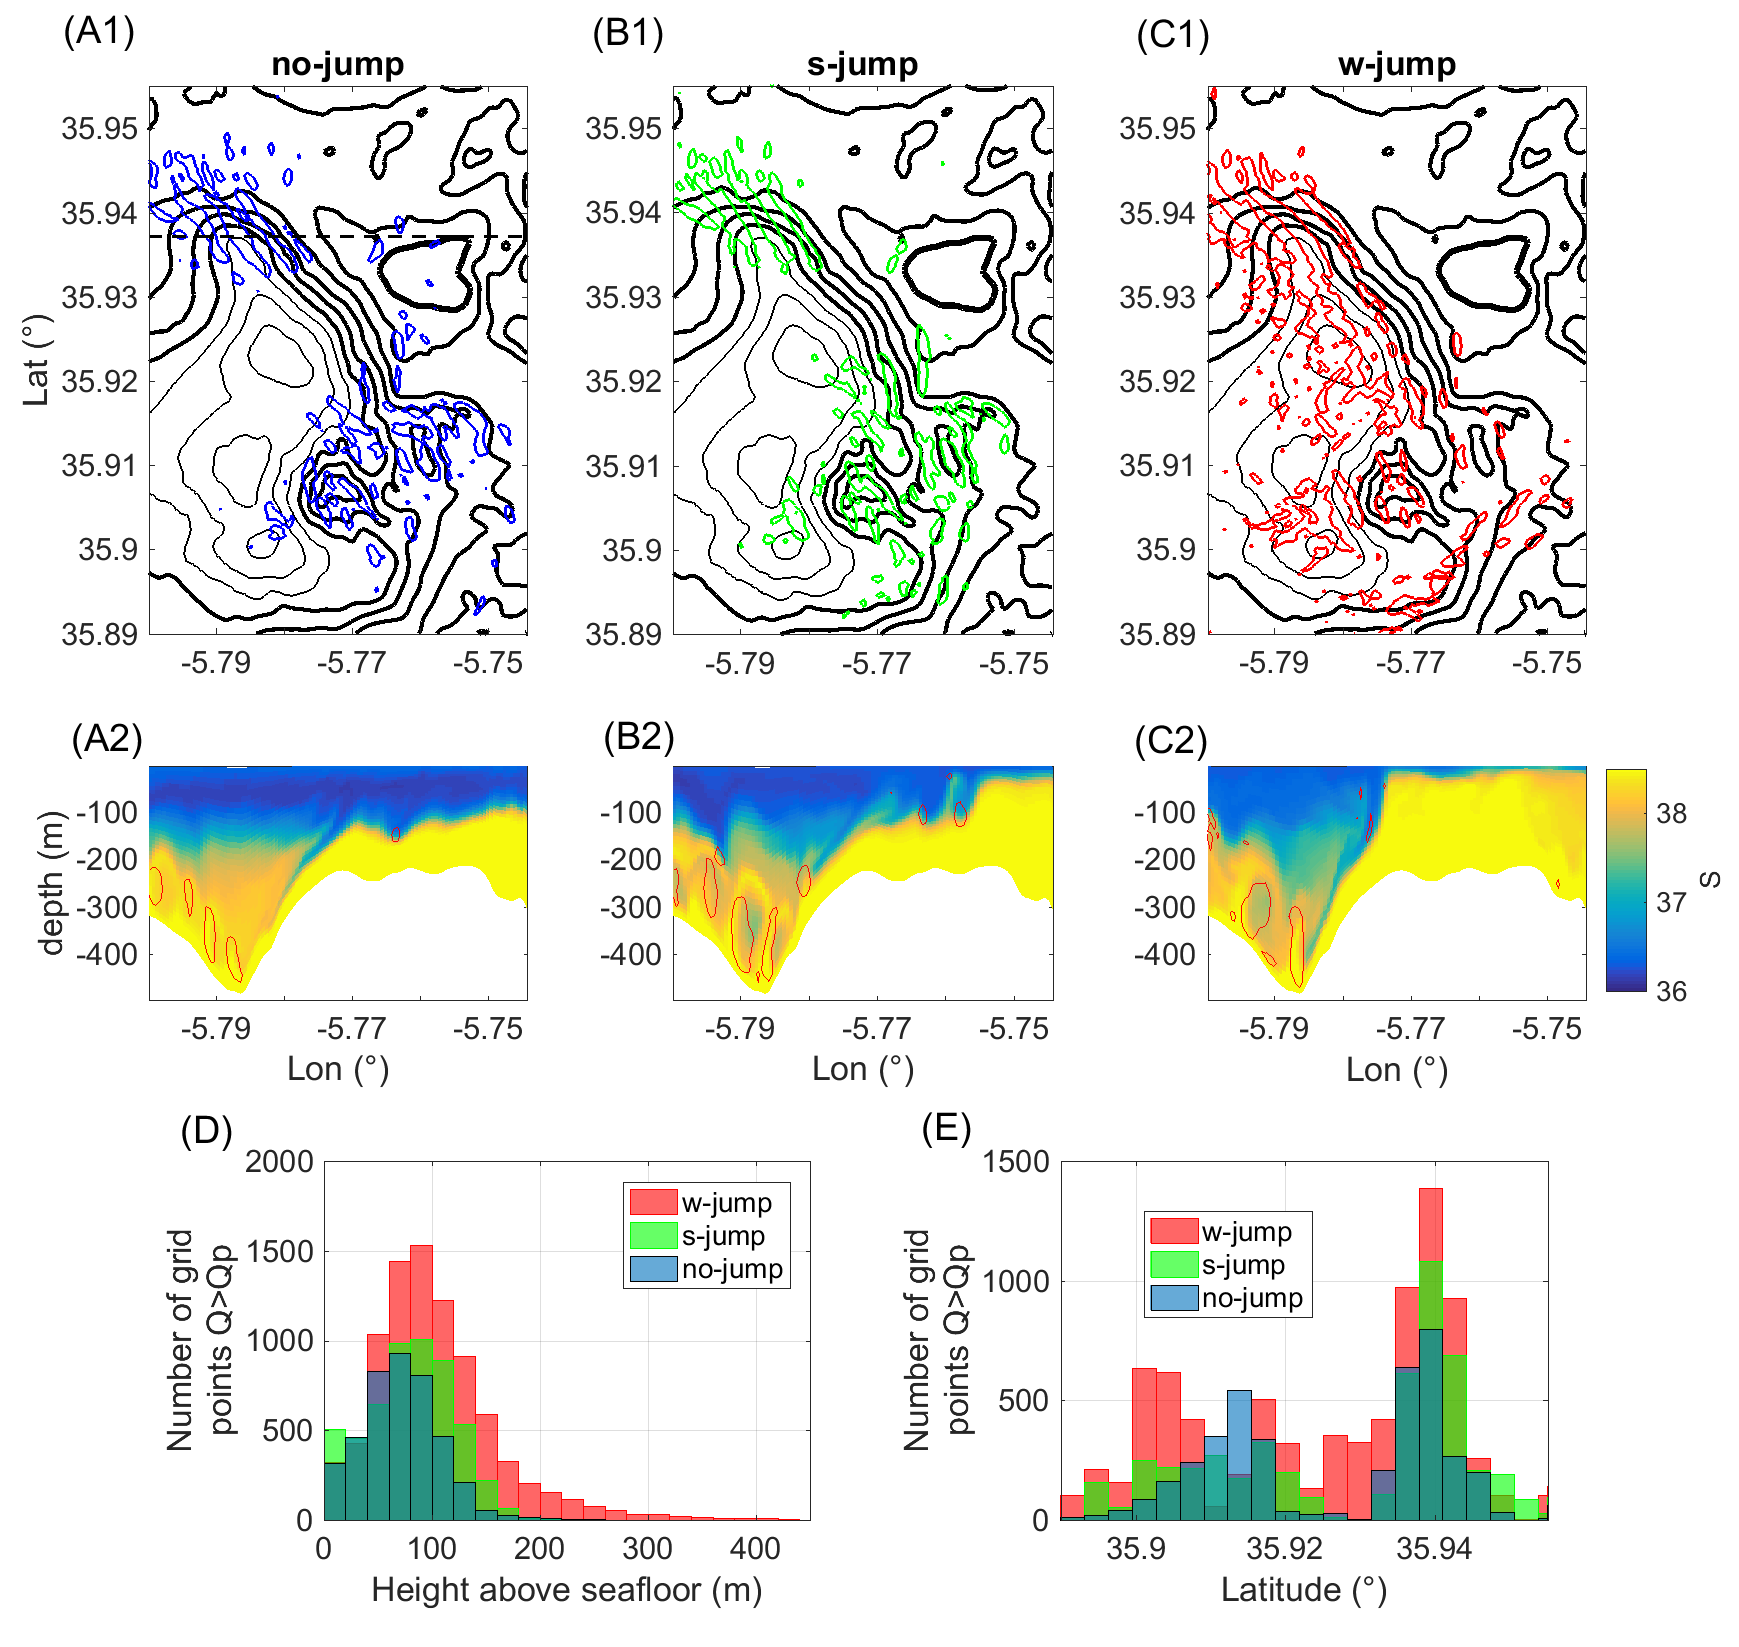
\includegraphics[width=\textwidth]{./GBR3D/EOF5_MIV_2D.png}
 \caption {(a, b, c) Contours of parameter Q$\ =\ 5.10^{-5}$ in first high-frequency EOF of SVD performed during outflow of figures \ref{FigHCN}.b,\ref{FigHCI} and \noparref{FigHCS}.b respectively. Isobathes (black) (200m, thicker)  (250 to 450, thick) (500 to 600m, thin). (d, e, f) vertical sections of salinity (color) and contours of Q-parameter $\ =\ 5.10^{-5}$ at latitude $35.9372^\text{o}$ at the same date and time as figures \noparref{FigHCN}.b,\ref{FigHCI} and \noparref{FigHCS}.b respectively. (g) histogram of the height of the grid points of each EOF shown in a, b and c above the seafloor. (h) histogram of the latitude of the grid points of each EOF shown in a, b and c above the seafloor.}
 \label{FigEOFMIV}
\end{figure}

 \color{green} Arrêt ici pour la première relecture Francis \color{black}

\subparagraph{Closure scheme}

\color{blue}\sout{Now look at four other simulations, three use Smagorinsky turbulent scheme with different coefficients. One is using GLS K-$\epsilon$. .}
Four additional simulations are now presented to investigate and better understand the impact of the turbulent scheme: the first three are based on a different implementation of the Smakorinsky turbulent scheme and the latest uses the GLS K-$\epsilon$ scheme. \color{black}
\color{blue}In figure \noparref{Fig3Dsch}.a, c, e and g),\color{black} vertical sections of salinity during the first outflow \color{blue}after $t\ =\ 5\ h$ \color{black} of simulation which is in a \textit{no-jump} case, with indications of the values of the Richardson gradient number $Ri$ and Q parameter. $Ri$ is calculated from fields of density and velocity averaged over half and hour to filter out the propagating structures.

\color{blue}Figures (\noparref{Fig3Dsch}.b, d, f, and h) show the averaged salinity in Mediterranean (b, f) and Atlantic layers (d, h) east (f,h) and west (b,d) \color{black} of CS. Note that averaged values are given and, as shown in figure \ref{FigTSCS} and in the vertical sections, the outflow Mediterranean layer is far from homogeneous at this longitude and at those longitudes. \color{black} \color{green}J ne suis pas sûr d'avoir bien rendu ce que tu voulais dire ici? \color{black}

Looking at averaged layer salinities  \color{green}(tu veux dire lorsque les salinités sont moyennées sur la couche, c'est cela?) \color{black} east of the sill in figures (\noparref{Fig3Dsch}.f and h), simulations SimIT-S001, SimIT-S01 and SimIT-Kep \color{blue} lead to the same salinities for the Mediterranean layer, whereas differences can be observed punctually in the Atlantic layer. The simulation presenting the largest differences is SimIT-S1: the Mediterranean layer is less saltier whereas the Atlantic layer is in contrast saltier. This is a direct consequence of the enhanced mixing coefficient which enhances in the pycnocline the mixing of these water masses. \color{black}

\color{blue}However west of the sill in SimIT-S1, whereas the Atlantic layer is still saltier so is the Mediterranean layer this time, especially between 2 and 8 hours following the initialization. This cannot obviously be explained by an increase of the dissipation.\color{black} After 5 hours of simulation, the vertical section shows that instabilities develop.  \color{blue}However, whereas the area of $Ri$ is lower than $1/4$ begins at 5.77$^\text{o}$ for all four simulations, indicating shear instabilities could develop from this point in the gravity current, we can ote that instabilities can be found down slope of an intrusion of Atlantic waters at 5.783$^\text{o}$ W in simulation SimIT-S1. \color{black}
\sout{While the other simulations, the salinity entrained by the billows is from the altantic layer//contain less salty waters, ie the signal of atl surface water in the med outflow will be stronger in this simulation.} \color{green}(while ? do you mean unlike or in contrast..?) \color{black}
 \color{blue}In contrast to the other simulations, the billows are made of Atlantic water and, as a consequence, they are less salty. \color{black}
 
\color{blue}A larger proportion of Atlantic water is also incorporated in the bellows when $K-\epsilon$ turbulent scheme is implemented. \sout{Kepsilon}. Indeed, in this case the billows and more generally the instabilities are less-developped \sout{instabilitied} with smaller values of parameter Q  \sout{(closer to a gravity current only?) ???}, and a less-salty outflow. This signal persists  \color{blue}$7\ h$ after the initialization when the flow reverses and no instabilities are generated any more. This process an also be observed but in a lesser extent in SimIT-S1 for which the effect of an increase diffusion in the pycnocline may counteract the injection of Mediterranean water. \color{black}

\sout{While} \color{blue}In simulations 1 and 2  \color{green}1 \& 2? \color{blue}, the width of the salty Mediterranean vein remains the same as it begins to go down slope of CS but instabilities arise earlier in the hydraulic jump and they bring more Atlantic water in the resulting billows. As these billows are advected down slope, more Atlantic water is integrated to the Mediterranean outflow when going through CS. \color{black} 


\begin{figure}[!h]
% \centering
 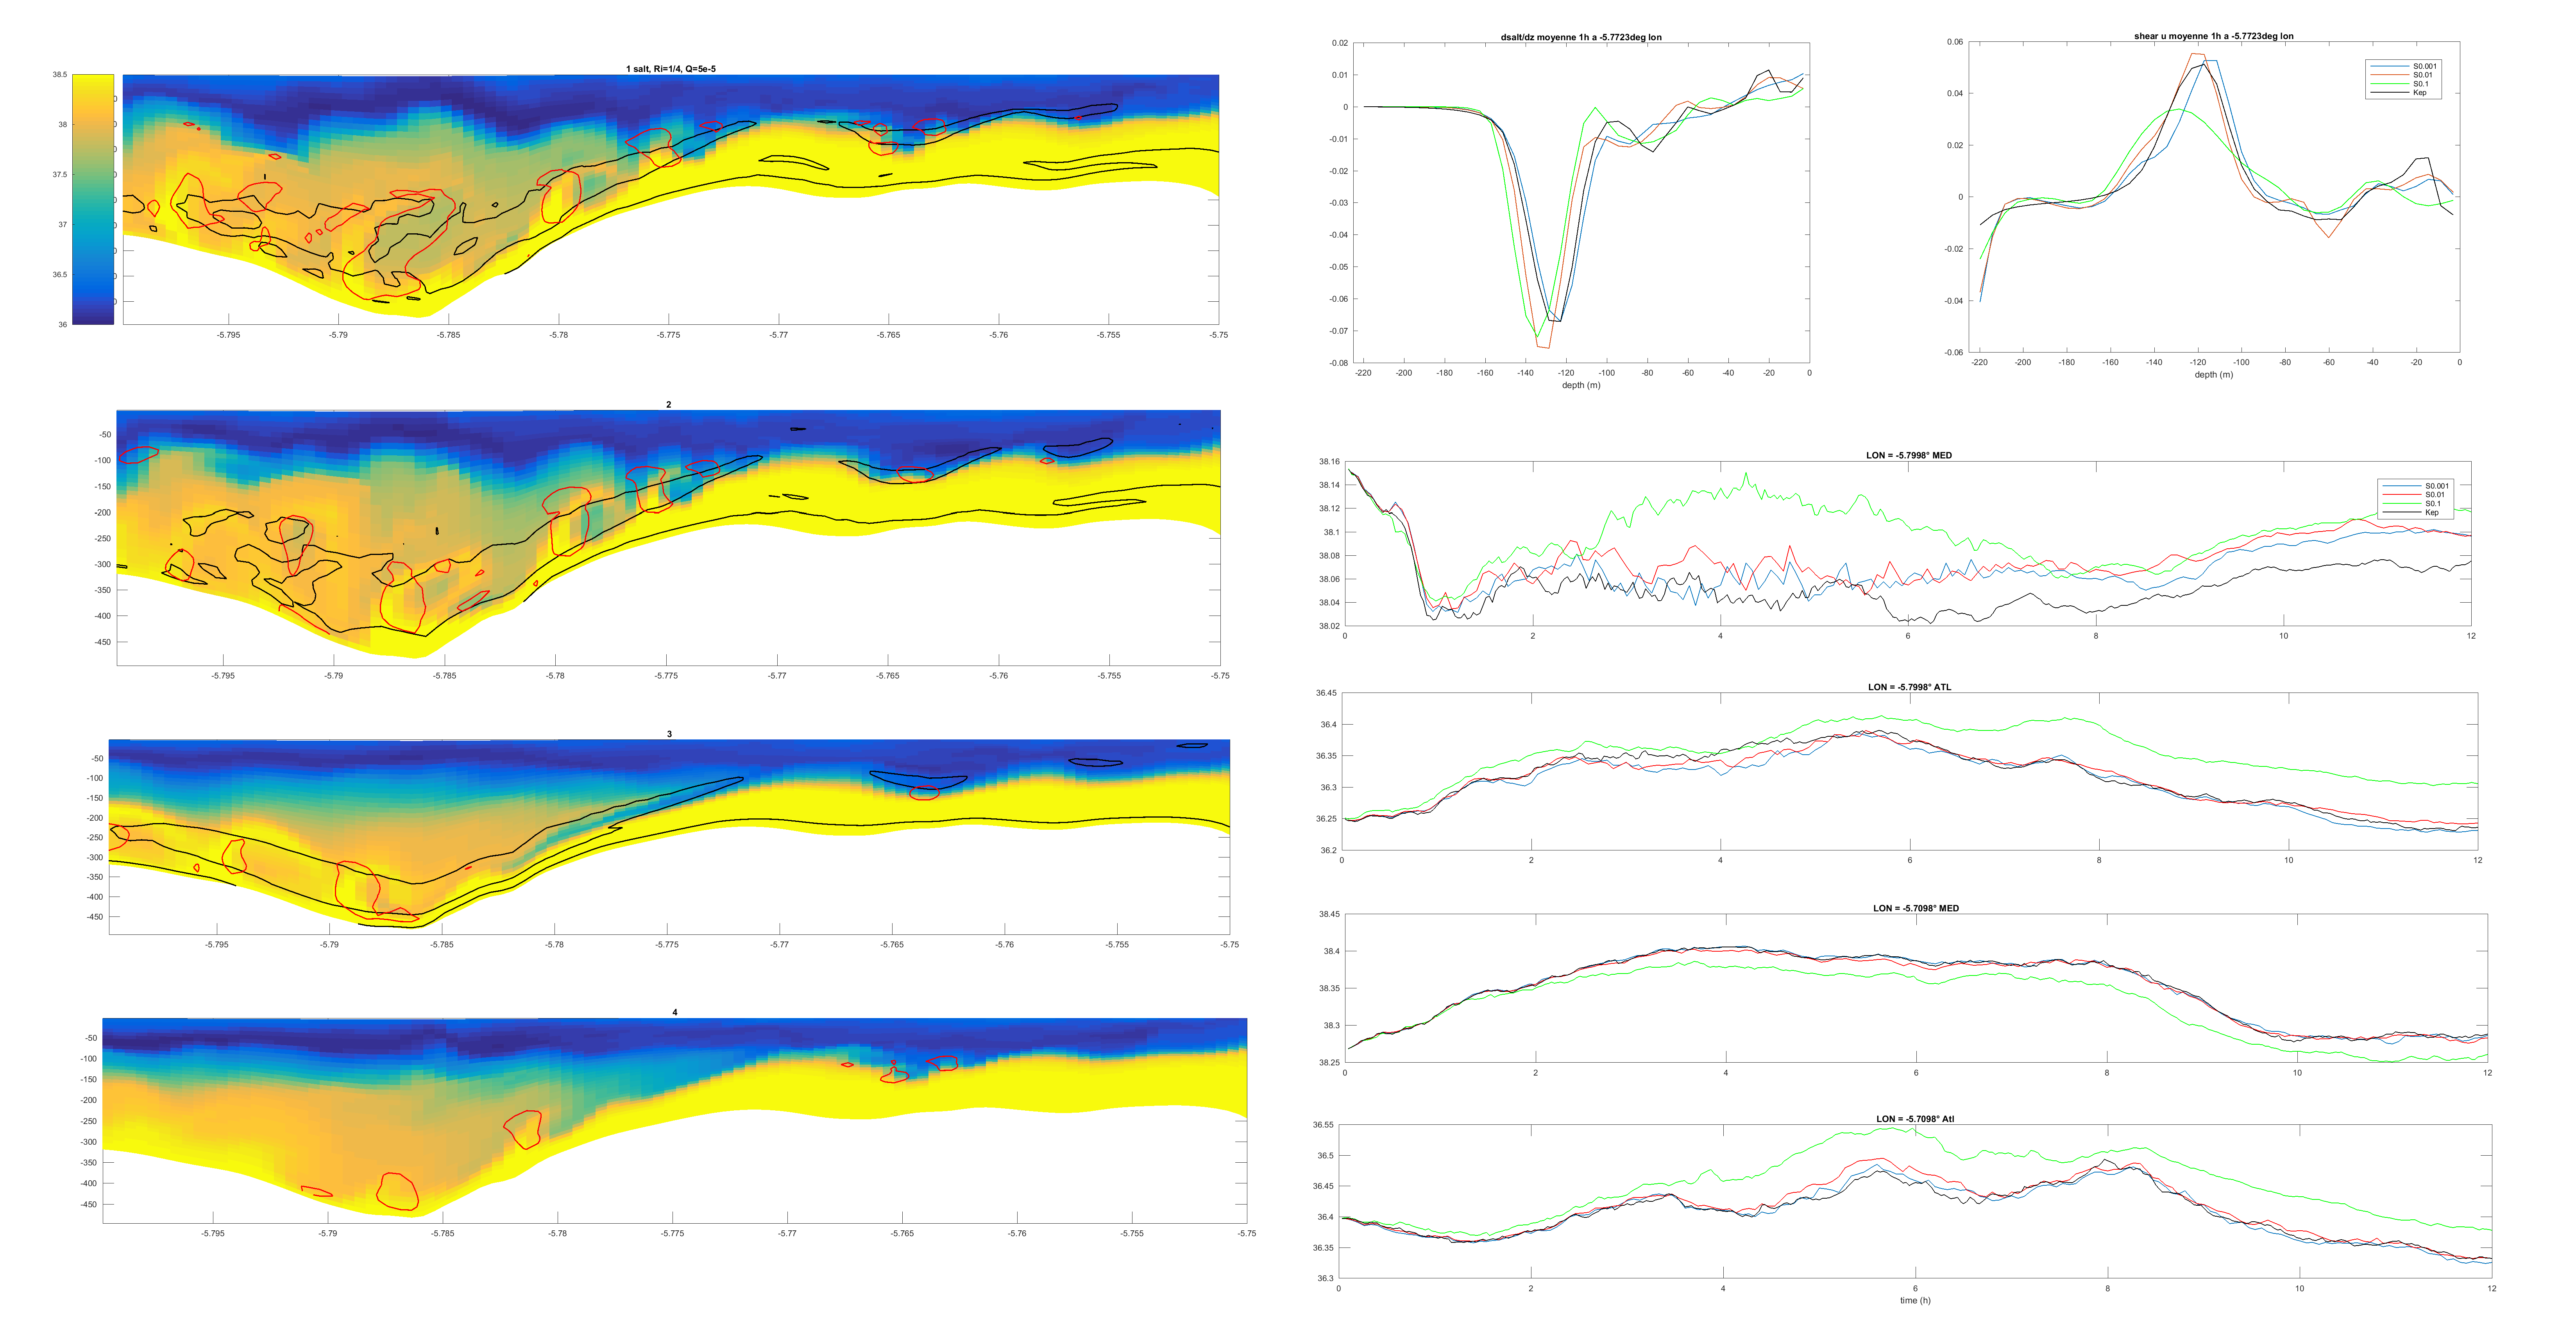
\includegraphics[width=\textwidth]{./GBR3D/Figsmago.png}
 \caption { \color{blue}vertical section of salinity (color), contours of $Q=5.10^{-5}$ (red) and Richardson gradient number $=\ 1/4$ (black) at a latitude of $35.9372^o\ N$ in SimIT-S001, SimIT-S01, SimIT-S1 and SimIT-Kep IES, 4 h after the initialization.  \color{green}time  (1:S0.001  2:S0.01  3:S0.1 4:Kep)(Rajouter une évolution de ubar!!! sur s0.001) Je te laisse rédiger la fin. \color{black}}
 \label{Fig3Dsch}
\end{figure}

%-------------------------------------------------------------------------------------
\section{Conclusion}

 \color{blue}\sout{Have looked into} The variability of the hydraulic control and of the other dynamical features during the neap-spring tidal cycle have been explored with high resolution, non-hydrostatic, free-surface simulations of the region of the strait of Gibraltar. \sout{.See no permanent} No permanent supercritical flow has been identified in the various simulations and only intermittent events of such flows have been observed during the tidal cycle, with location and extension of the area of supercritical flow depending on the strength of the barotropic currents. \color{black}
\color{blue}During outflows when both Atlantic and Mediterranean layers are critical, an hydraulic jump is generated and explicitly simulated. They are located \color{black} either over the shallowest part of the sill, or over its western slope.  \color{blue}This hydraulic jump evolves into a train of solitary waves, as can be expected when the hydraulic control stops close to high tide. The train of solitons finally leaves the strait into the Alboran Sea. 
During tidal cycles with no critical flow over the sill and no hydraulic jump, the barotropic tidal signal induces a less extended train of solitary waves in the eastern part of the strait due to non-linearity. This train propagates into the Alboran Sea.  \color{green}J'ai eu du mal à comprendre, est-ce bien ce que tu voulais dire? \color{black}

 \color{blue}During \color{black} each simulated tidal cycle, a cyclonic eddy is formed of the coast of Ceuta in the southern part of the eastern exit of the Strait. This eddy is advected by the flow in the Alboran Sea and interacts with the train of solitary waves, \color{blue}inducing a local diffraction of the solitons. \color{black}


\color{blue}Several other dynamical features have been explicitly simulated such as the billows resulting from shear instabilities and developing\color{black} in the lee of CS. In simulations, these billows are associated with high positive values of parameter Q which is used as proxy for their detection and analysis. The billows are generated at the interface of \color{blue} Mediterranean and Atlantic waters and they are advected by the Mediterranean outflow. They are also present above secondary bathymetry accidents in Tangier basin and ES. They can be observed during outflows of any intensity, but their spreading changes with the intensity of tidal currents. They play an important role in the way Mediterranean and Atlantic waters mixe in the simulation, changing the hydrological features of the Mediterranean vein. The way this mixing occurs in simulations is sensitive to the dynamic of the instabilities and this dynamic is piloted by the turbulent dissipation scheme. \color{black}

\sout{Can see that} \color{blue}A conclusion is that the hydrological and dynamical properties of the Mediterranean waters entering in the Nothern Atlantic basin are greatly affected by the configuration of the fow in the region of CS. Both the volume of these Mediterranean waters and their mixing with Atlantic waters can indeed vary during the neap-tide cycle. \color{black}
%the configuration of the flow at CS is the first passage of the Med waters, will affect the hydrological properties of the Mediterranean outflow, first by the volume of med waters that can flow west of the sill at each outflow, second by how much Atlantic waters are being mixed into it. 

%However, it is important to note that simulation only represents the beginning of the mixing by turbulent processes, in particular, no secondary evolution of KH instabilities.
\color{blue}In the present numerical configurations, only the largest primary instabilities and thus only the upper part of the turbulent direct cascade were explicitly simulated. The route to mixing consequently depends on the quality of the turbulence closure scheme used to end up mixing the water masses and this dependency has been evaluated by testing several schemes with well-known properties. The present work is thus a first LES\footnote{LES: Large Eddy Simulation} exploration in \textit{Terra Incognita} \cite{scotti_large_2010;wyngaard_toward_2004}.\color{black}


%Moreover, the lack of atmospheric forcing probably means inaccuracies of features of the upper layer, especially circulation of the Atlantic layer in Tarifa Narrows where wind stress affects the upper layer. 
\color{blue}No atmospheric forcing were specified at the surface of the ocean in configurations presented in this section. This means that the upper layer is not realistically represented in particular in the region of Tarifa Narrows where wind stress is particularly strong. This choice remains yet consistent with the desire to simplify (but not over simplify) the fine-structure dynamic in the complex region of the strait of Gibraltar. \color{black}

This choice could moreover explain why have the baroclinic tide degenerate into an internal bore and then into a train of solitary waves during any inflows following a \textit{no-jump} outflow at CS, whereas observations \color{green}(cite tes sources) \color{black} indicate that during neap tides no solitary waves are generated. \color{green}(Ai-je bien compris ce que tu voulais dire ?). Other processes could be affected \color{blue} by the absence of atmospheric forcing \color{black} like the formation of eddies at the exit of the strait and their advection into \color{blue}the Alboran sea \color{black} that is probably influenced by the WAG.
